\documentclass[]{elsarticle} %review=doublespace preprint=single 5p=2 column
%%% Begin My package additions %%%%%%%%%%%%%%%%%%%
\usepackage[hyphens]{url}



\usepackage{lineno} % add
\providecommand{\tightlist}{%
  \setlength{\itemsep}{0pt}\setlength{\parskip}{0pt}}

\usepackage{graphicx}
\usepackage{booktabs} % book-quality tables
%%%%%%%%%%%%%%%% end my additions to header

\usepackage[T1]{fontenc}
\usepackage{lmodern}
\usepackage{amssymb,amsmath}
\usepackage{ifxetex,ifluatex}
\usepackage{fixltx2e} % provides \textsubscript
% use upquote if available, for straight quotes in verbatim environments
\IfFileExists{upquote.sty}{\usepackage{upquote}}{}
\ifnum 0\ifxetex 1\fi\ifluatex 1\fi=0 % if pdftex
  \usepackage[utf8]{inputenc}
\else % if luatex or xelatex
  \usepackage{fontspec}
  \ifxetex
    \usepackage{xltxtra,xunicode}
  \fi
  \defaultfontfeatures{Mapping=tex-text,Scale=MatchLowercase}
  \newcommand{\euro}{€}
\fi
% use microtype if available
\IfFileExists{microtype.sty}{\usepackage{microtype}}{}
\usepackage[left=3cm,right=3cm,top=3cm,bottom=3cm]{geometry}
\bibliographystyle{elsarticle-harv}
\usepackage{longtable}
\ifxetex
  \usepackage[setpagesize=false, % page size defined by xetex
              unicode=false, % unicode breaks when used with xetex
              xetex]{hyperref}
\else
  \usepackage[unicode=true]{hyperref}
\fi
\hypersetup{breaklinks=true,
            bookmarks=true,
            pdfauthor={},
            pdftitle={Living on the edge: crop boundary effects on precision crop yields in Alberta, Canada},
            colorlinks=false,
            urlcolor=blue,
            linkcolor=magenta,
            pdfborder={0 0 0}}
\urlstyle{same}  % don't use monospace font for urls

\setcounter{secnumdepth}{5}
% Pandoc toggle for numbering sections (defaults to be off)

% Pandoc citation processing
\newlength{\csllabelwidth}
\setlength{\csllabelwidth}{3em}
\newlength{\cslhangindent}
\setlength{\cslhangindent}{1.5em}
% for Pandoc 2.8 to 2.10.1
\newenvironment{cslreferences}%
  {}%
  {\par}
% For Pandoc 2.11+
\newenvironment{CSLReferences}[3] % #1 hanging-ident, #2 entry spacing
 {% don't indent paragraphs
  \setlength{\parindent}{0pt}
  % turn on hanging indent if param 1 is 1
  \ifodd #1 \everypar{\setlength{\hangindent}{\cslhangindent}}\ignorespaces\fi
  % set entry spacing
  \ifnum #2 > 0
  \setlength{\parskip}{#2\baselineskip}
  \fi
 }%
 {}
\usepackage{calc} % for calculating minipage widths
\newcommand{\CSLBlock}[1]{#1\hfill\break}
\newcommand{\CSLLeftMargin}[1]{\parbox[t]{\csllabelwidth}{#1}}
\newcommand{\CSLRightInline}[1]{\parbox[t]{\linewidth - \csllabelwidth}{#1}}
\newcommand{\CSLIndent}[1]{\hspace{\cslhangindent}#1}

% Pandoc header
\makeatletter \def\ps@pprintTitle{  \let\@oddhead\@empty  \let\@evenhead\@empty  \def\@oddfoot{\centerline{\thepage}} \let\@evenfoot\@oddfoot} \makeatother \usepackage{float} \floatplacement{figure}{H} \newcommand{\beginsupplement}{\setcounter{table}{0} \renewcommand{\thetable}{S\arabic{table}} \setcounter{figure}{0} \renewcommand{\thefigure}{S\arabic{figure}}} \usepackage{setspace} \linenumbers
\usepackage{booktabs}
\usepackage{longtable}
\usepackage{array}
\usepackage{multirow}
\usepackage{wrapfig}
\usepackage{float}
\usepackage{colortbl}
\usepackage{pdflscape}
\usepackage{tabu}
\usepackage{threeparttable}
\usepackage{threeparttablex}
\usepackage[normalem]{ulem}
\usepackage{makecell}
\usepackage{xcolor}



\begin{document}
\begin{frontmatter}

  \title{Living on the edge: crop boundary effects on precision crop yields in Alberta, Canada}
    \author[University of Calgary]{Samuel V. J. Robinson\corref{1}}
   \ead{samuel.robinson@ucalgary.ca} 
    \author[University of Calgary]{Lan H. Nguyen}
   \ead{hoanglan.nguyen@ucalgary.ca} 
    \author[University of Calgary]{Paul Galpern}
   \ead{paul.galpern@ucalgary.ca} 
      \address[University of Calgary]{2500 University Drive NW, Calgary, AB}
      \cortext[1]{Corresponding Author}
  
  \begin{abstract}
  Field boundaries can improve crop yields by creating better abiotic conditions for crop growth (e.g.~moisture, temperature), and can act as refuges for beneficial arthropods. This suggests that beneficial crop boundaries may create an intermediate hump-shaped increase in crop yield, where negative edge effects are cancelled out by increased ecosystem services (e.g.~pollination or pest suppression) from the field boundary. However, there is little large-scale evidence showing this, largely because yield is costly and time-consuming to measure. Precision yield data from combine yield monitors has huge potential in this respect, as the equipment is relatively cheap and commonly measured by growers. In this study, we used 252 field-years of yield monitor data from three common crops -- wheat (\emph{Triticum aestivum}), canola (\emph{Brassica napus}), or peas (\emph{Pisum sativum}) -- recorded across Alberta, Canada, and examined how yield varied with distances from common crop boundary types. Average crop yield tended to increase with distance from crop boundaries before plateauing at about 50 m, and yield variation (SD) tended to decrease with distance. There was evidence of an intermediate increase in yield for wheat away from shelterbelts, and a weak increase in canola, but no other boundary type showed evidence of this. This study represents one of the first uses of precision yield data to measure ecosystem service provision at large spatial scales.
  \end{abstract}
   \begin{keyword} precision yield; spillover; landscape;\end{keyword}
 \end{frontmatter}

Potential journals: Agriculture Ecosystems and Environment, Basic and Applied Ecology, Ecological Economics, Journal of Applied Ecology (probably won't like it)

Potential reviewers: Teja Tscharntke, Ignasi Bartomeus, Ben Woodcock, John Redhead, some Canadian/Albertan reviewers who know the crop systems?

\newpage
\doublespacing

\hypertarget{introduction}{%
\section{Introduction}\label{introduction}}

Intensive agricultural production has increased over the last 100 years, and agricultural land now makes up over a third of ice-free land on Earth (Ramankutty \emph{et al.} 2018).
This has allowed increases in human population and increased global stability in production (Foley \emph{et al.} 2011).
However, this is not without cost, as higher-diversity non-crops are converted to lower-diversity crops, resulting in loss of habitat and overall biodiversity of non-target organisms.
Maintaining both biodiversity and production in agroecosystems represents a goal of conservationists and agronomists, and holds the potential for win-win scenarios ({``multifunctionality''} \emph{sensu} Mitchell \emph{et al.} 2014; Frei \emph{et al.} 2018).
Key to this goal is the preservation of semi-natural land (SNL) in and around crops, which represents the interface between crops and non-crops within agroecosystems.

SNL in agroecosystems is important for both agricultural production and conservation (Prieto-Benítez \& Méndez 2011), and can create better biotic and abiotic conditions for crop growth (Case \emph{et al.} 2019; Weninger \emph{et al.} 2021; but see Lowe \emph{et al.} 2021).
SNL constitutes habitat for mobile organisms, and can act as sources of ecosystem services such as pollination or pest control (Albrecht \emph{et al.} 2020; Gardner \emph{et al.} 2021), but this can vary depending on the crop system (Gray \& Lewis 2014; Quinn \emph{et al.} 2017) and landscape context (Marja \emph{et al.} 2019; Boetzl \emph{et al.} 2020).
They also can create microclimate effects that reduce extreme temperature, trap moisture, and reduce wind speed and soil erosion (Kort 1988; Brandle \emph{et al.} 2004; Wratten \emph{et al.} 2012).
North American agroecosystems have larger fields, different crop varieties, and agronomic practices, all of which could negate or confound potential effects of SNL.
Semi-natural field boundaries (e.g.~grass and flower strips, tree or shrub shelterbelts, road right-of-ways) are of particular interest, as they are extremely common and require less land than field-sized agricultural set-asides.

Field boundaries can cause both positive or negative effects on crops, depending on the spatial scale at which ecosystem services operate.
Low yields near may occur near the edge of the field because of patchy seed emergence, poor microclimate, shading from trees, or greater competition with weeds.
Field boundaries can also provide helpful ecosystem services, such as pest suppression or pollination, and these also tend to be occur close to the field edge (Duelli \& Obrist 2003).
For example, crop pollination services from bees that nest in field boundaries drops rapidly with distance (Kowalchuk \& Jong 1995; Garibaldi \emph{et al.} 2011).
If negative edge effects of the edge improve with distance and ecosystem services decrease with distance, yield may be maximized at intermediate distances where the ecosystem services cancel out negative edge effects {[}Mitchell \emph{et al.} (2014); Van Vooren \emph{et al.} (2017); Figure \ref{fig:hypotheses}a{]}.
This suggests a ``Goldilocks'' field size, where negative edge effects are canceled out by ecosystem services.
Alternatively, if ecosystem services are constant with distance (or increase, Figure \ref{fig:hypotheses}b) then yield will increase with distance from a field boundary and then plateau.

\begin{figure}
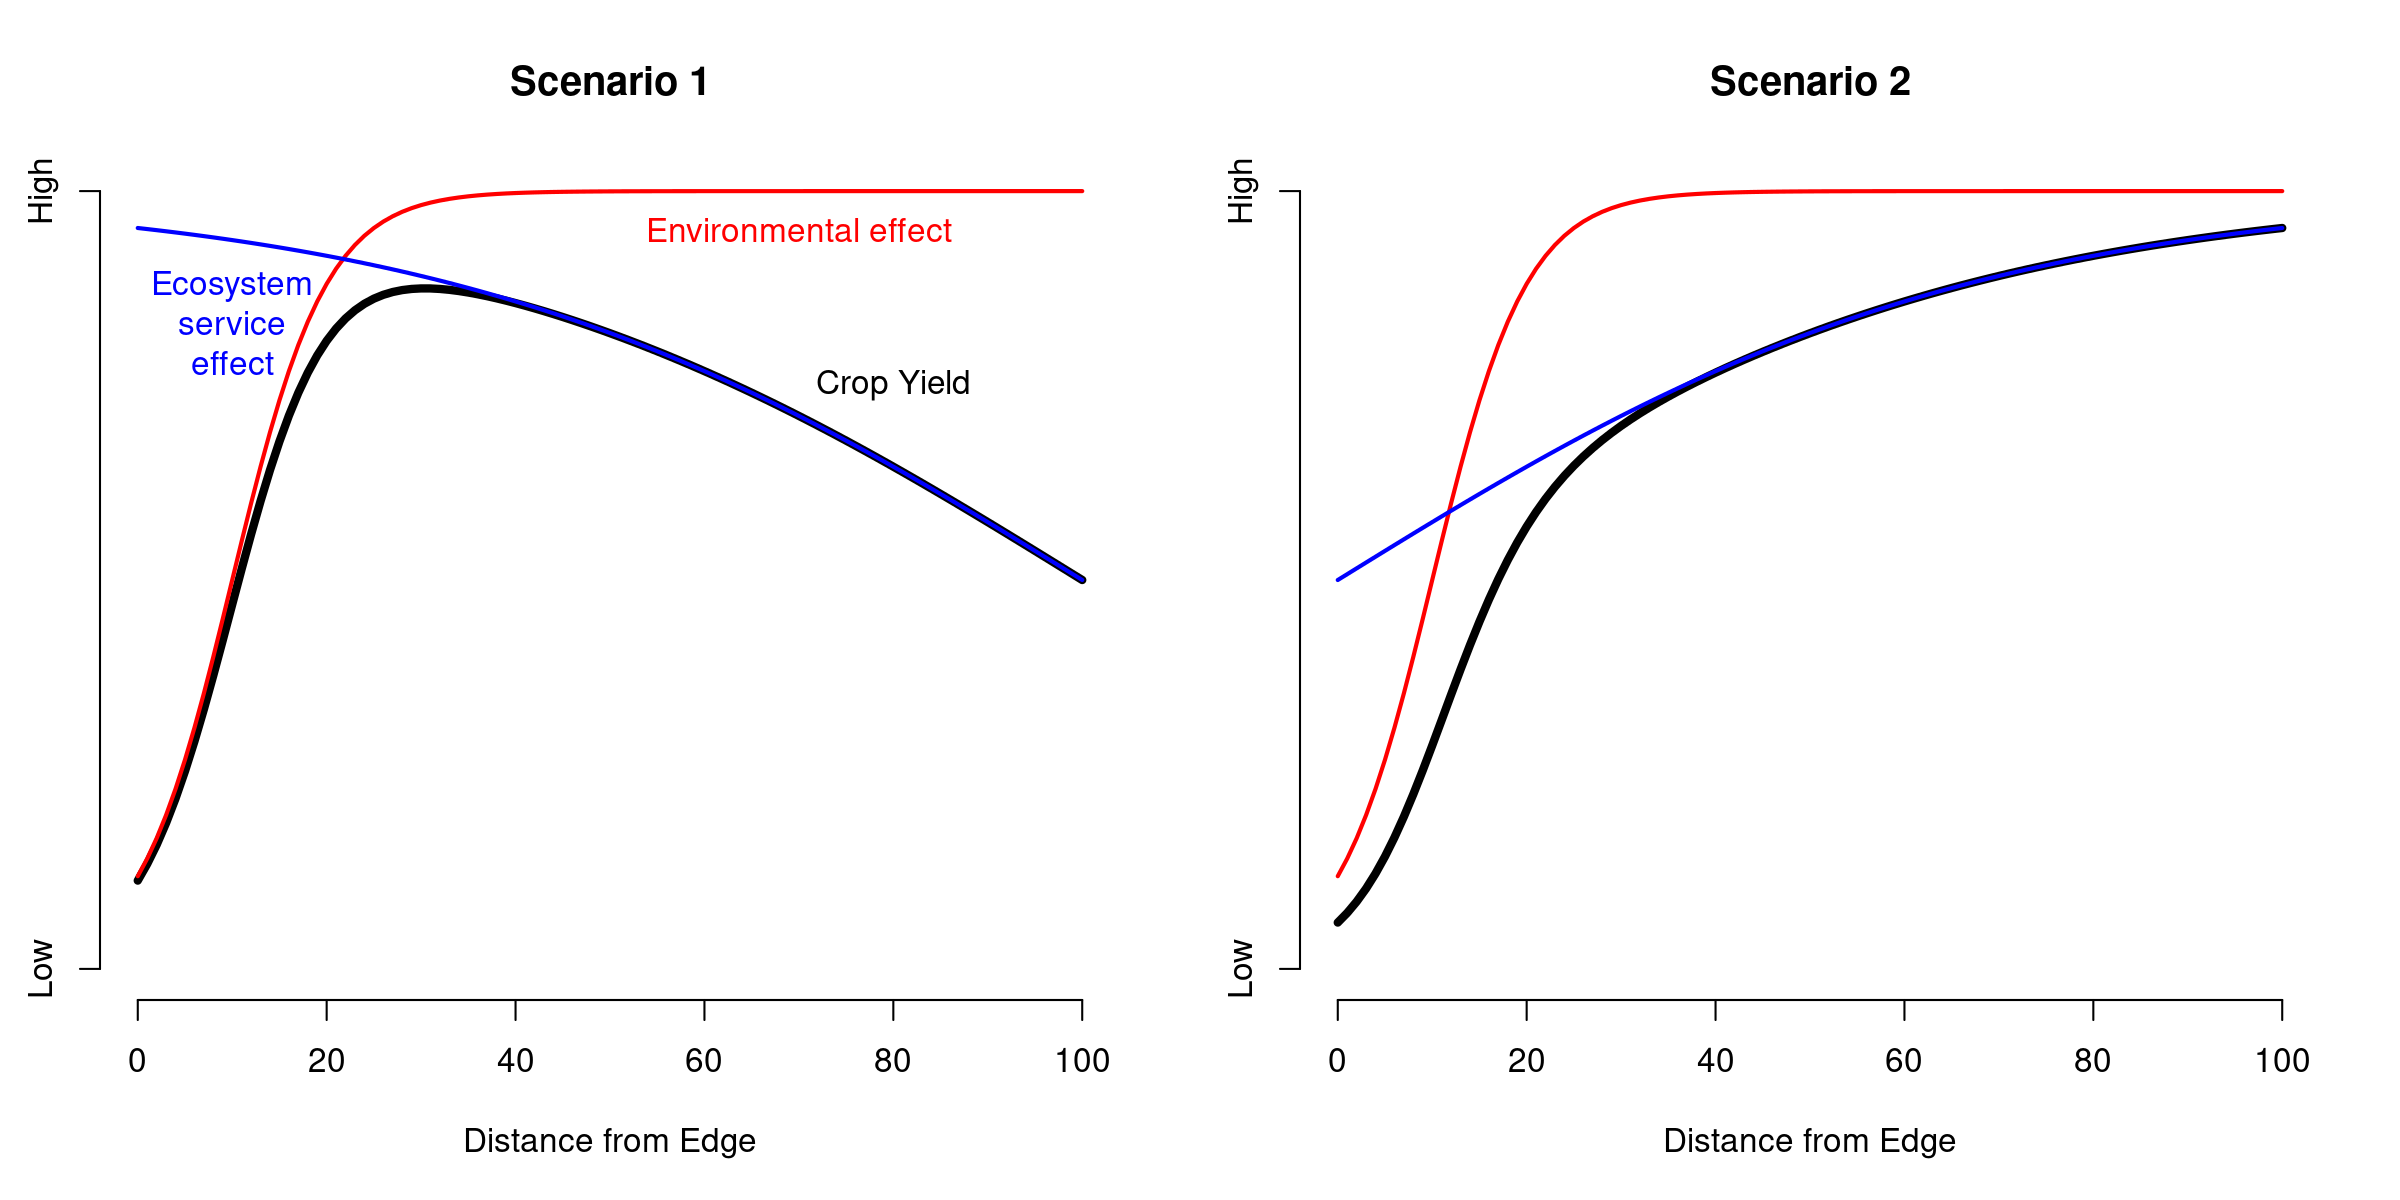
\includegraphics[width=1\linewidth]{../Figures/ExamplePlots/hypotheses} \caption{Potential yield patterns, depending on ecosystem service effects with distance. In both figures, negative environmental effects (edge effects) are shown in red, and decrease with distance from the edge of the crop, creating an increase in yield with distance. The left figure shows a decline in ecosystem services with distance, leading to an intermediate peak in yield, while the right figure shows an increase in services with distance, leading to a peak at the centre of the field (note: Scenario 2 also occurs if ecosystem services do not change with distance).}\label{fig:hypotheses}
\end{figure}

Boundary effects are difficult to observe without large amounts of crop yield data, which is typically expensive and time-consuming to collect.\\
Studies of semi-natural field boundaries on crop yield tend to suffer from limited spatial scope and small sample sizes, limiting inference and reducing generality (Baker \emph{et al.} 2018; but see also Redhead \emph{et al.} 2020).
Meta-analyses are a common solution to this problem (e.g. Albrecht \emph{et al.} 2020; Lowe \emph{et al.} 2021), but precision yield data holds enormous promise because of its relatively common usage and low operating costs.
However, its use is limited for several reasons, namely: 1) Lack of standardized formats between equipment types, 2) Sensor calibration required for field-level accuracy, and 3) low familiarity with spatial statistics.
Ecosystem services from field boundaries may influence both the mean as well as the variability of yield in agroecosystems (Redhead \emph{et al.} 2020; Hünicken \emph{et al.} 2021); typically only means are considered, but lower variability in yield can also be valuable from a grower's perspective.
There are few studies of yield variability (only those with large datasets), but precision yield data opens up the possibility of modeling within-field variability, as well as average yield.

In this paper use a precision yield dataset from Alberta, Canada to ask the following questions:
1. How does crop yield change with distance from the edge of field?
2. Does this depend on type of field edge?
3. Is there an intermediate distance where yield is maximized or variance is minimized?
To our knowledge, no other study has studied the effects of field boundaries using precision yield data, making this study one of the first of its kind.

\hypertarget{methods}{%
\section{Methods}\label{methods}}

\hypertarget{data-collection}{%
\subsection{Data collection}\label{data-collection}}

Precision yield data were collected directly from farmers across Alberta.
Farmers were solicited for yield data through local agronomists, and we received 298 field-years of data from 5 growers across a total of 7 years (2014-2020).
We converted raw data to a standard csv format using Ag Leader SMS®.
85\% of the crop types where either wheat (\emph{Triticum aestivum}), canola (\emph{Brassica napus}), or peas (\emph{Pisum sativum}), three of the most common crops in rotation in Alberta (Statistics Canada 2014).
The remaining crop types had low replication, so we constrained our analysis to only field-years containing wheat (91), canola (118), or peas (38), for a total of 247 field-years of data.
Individual fields contained between 1 and 6 years of data (mean: 3), containing a total of 13.9 million data points.

\begin{figure}
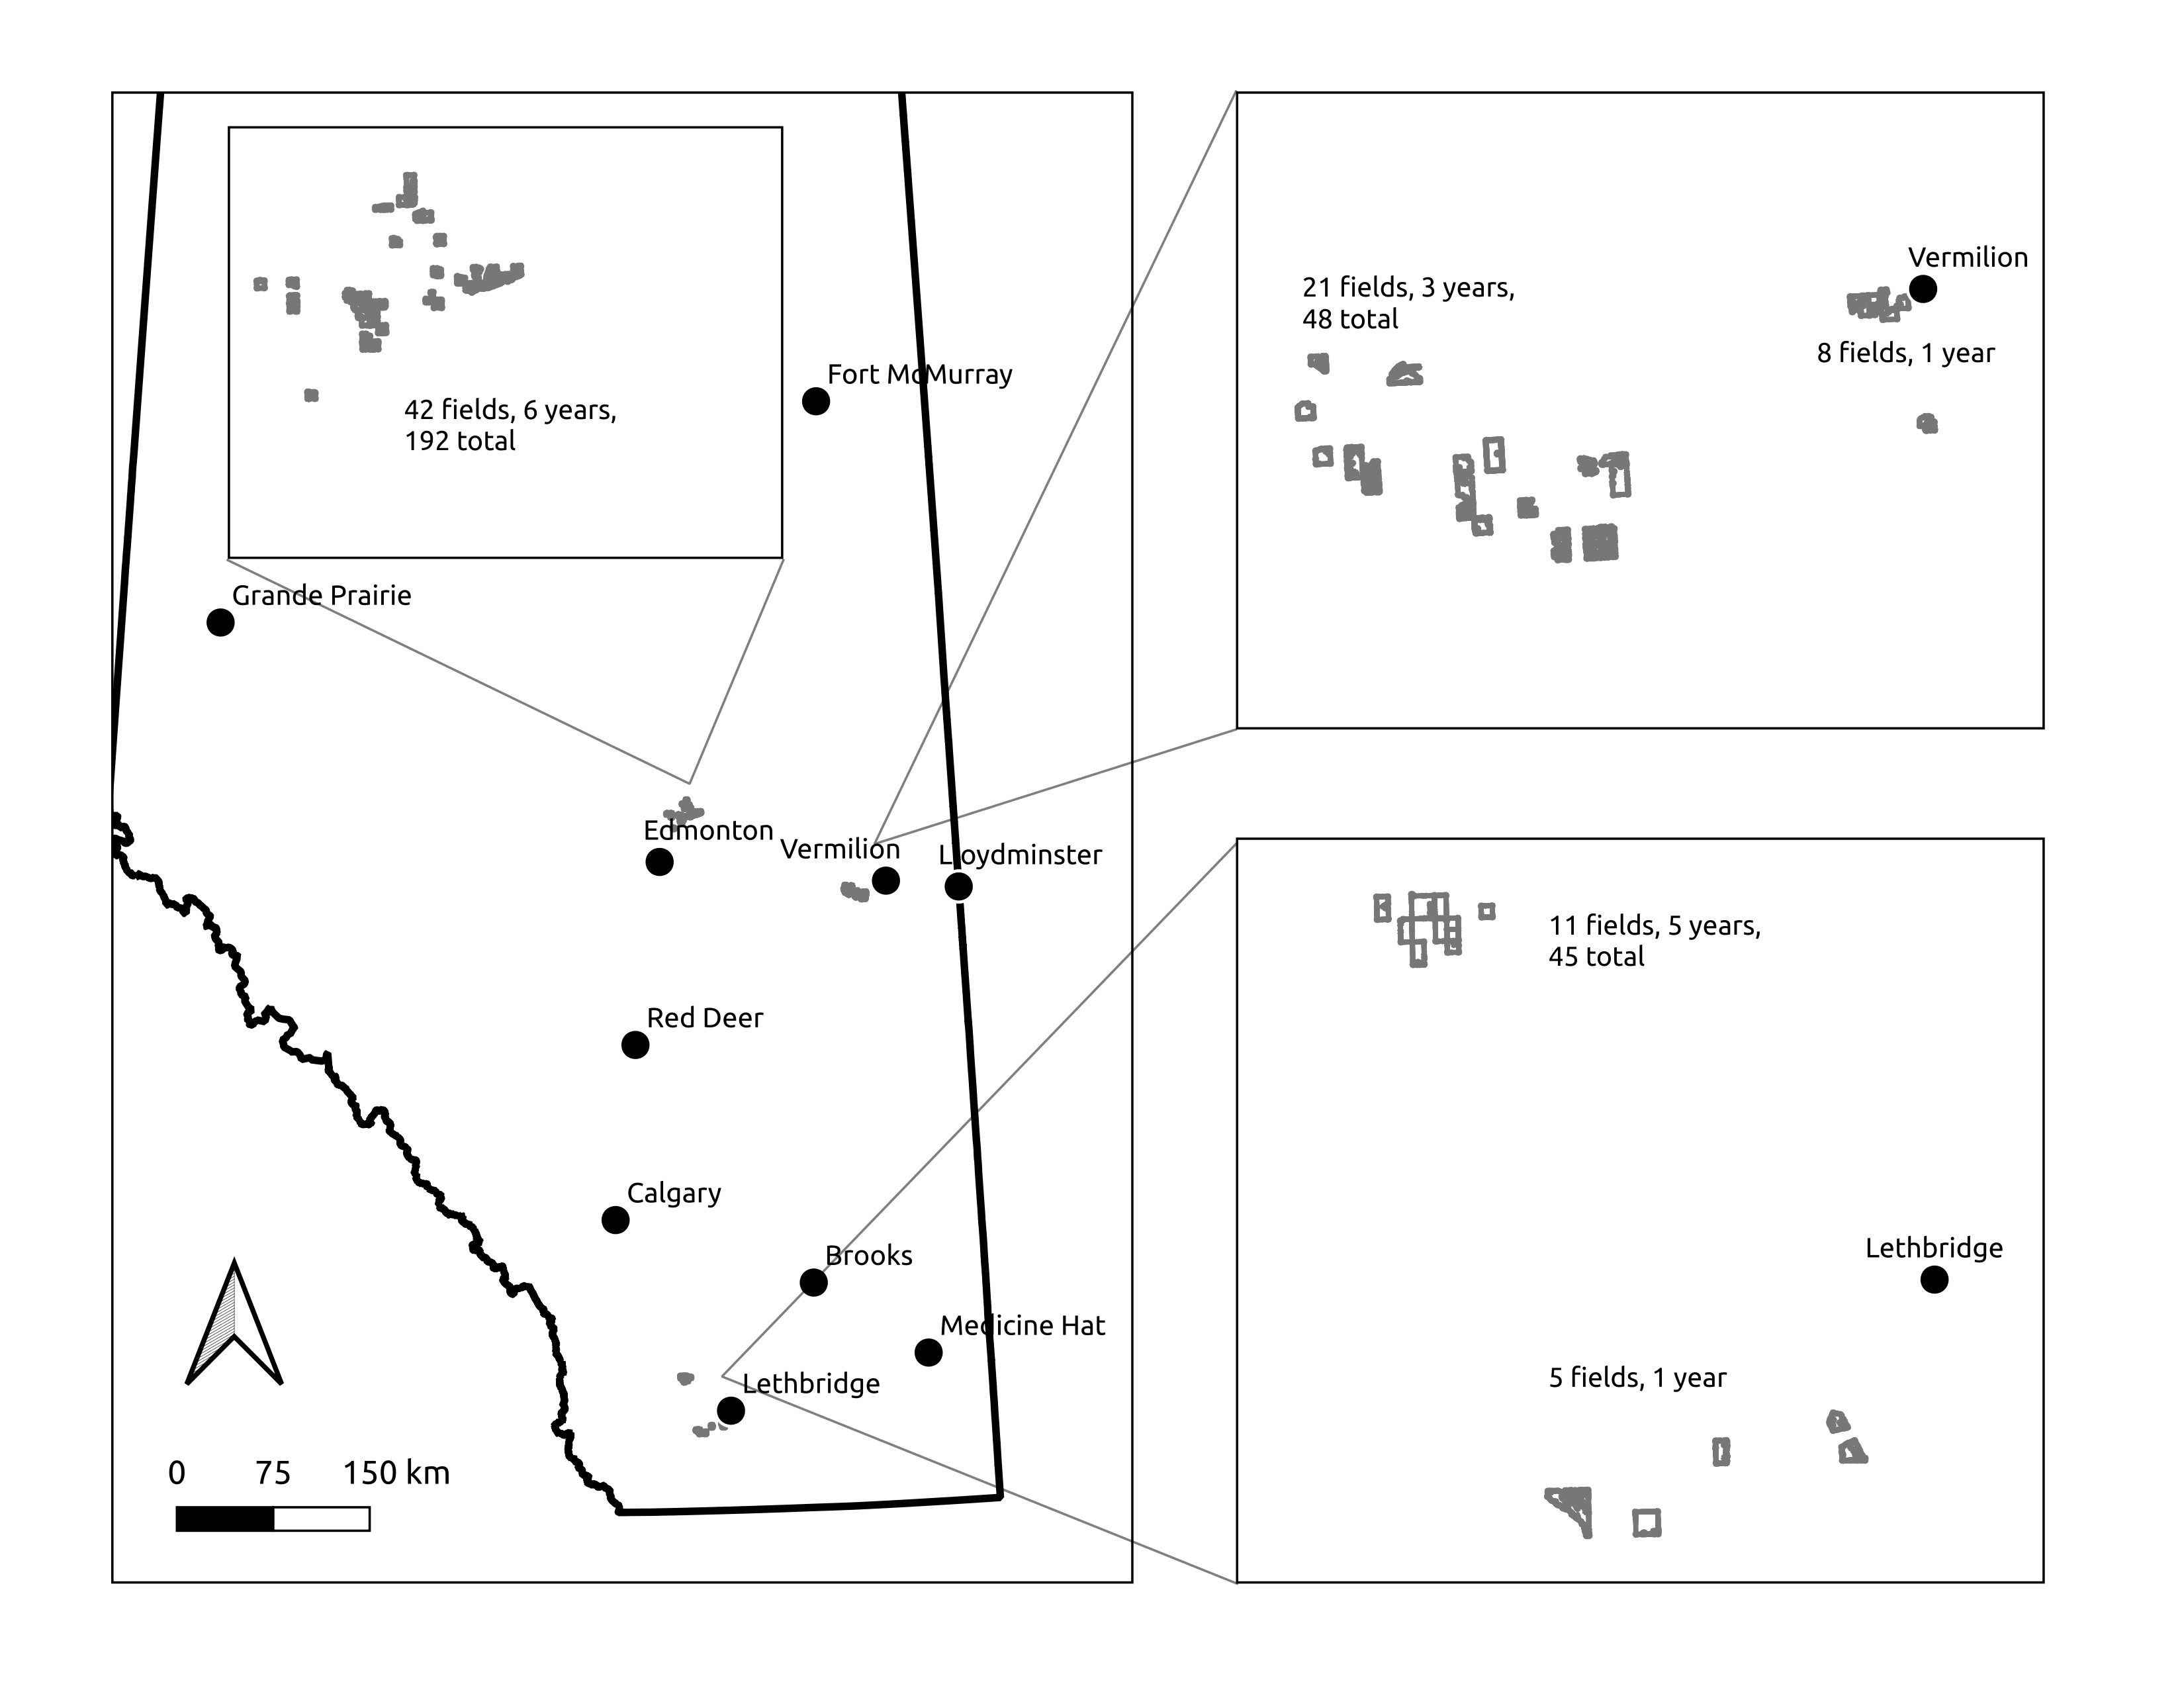
\includegraphics[width=1\linewidth]{../Figures/Field Locations} \caption{Locations of fields that data were collected from}\label{fig:fieldLocataions}
\end{figure}

Yield data was collected in rectangles of the same length as the data interval (distance = combine ground speed \(\times\) interval, typically 1 second) and the same width as the combine header (5-7 m, adjusted by the combine to account for overlap with adjacent swaths).
We used dry yield (tonnes of seed per hectare minus - crop moisture) as our measure of yield, using the size of each rectangle (m\(^2\)), dry yield (tonnes), and the spatial location.
Because of the large number of yield rectangles per field (30-800 thousand), we used the centroid of each polygon as its location, treating areal data as point data.
Seeding and application rates were constant across fields, so we did not consider inputs in our analysis.
Precision yield data can be highly variable and is prone to extreme outliers, especially when combine ground speeds are low and at the beginning of rows (Griffin \emph{et al.} 2007; Whelan \& Taylor 2013), or when the combine is accelerating or decelerating (Arslan \& Colvin 2002).
Therefore, we used the following filtering procedure to clean the data prior to model fitting:

\begin{enumerate}
\def\labelenumi{\arabic{enumi}.}
\tightlist
\item
  Removed outliers and ``inliers'' using the spatial filtering procedure from (Vega \emph{et al.} 2019)
\item
  Removed unrealistic yield values (10.75 T/ha for wheat, 8 T/ha for canola and peas), and values of zero or less
\item
  Removed extremely low and high outliers (below 1st percentile, above 99th percentile) for: dry yield, steering angle differences, ground speed
\item
  Removed points with large changes (\textgreater20\%) in ground speed
\item
  Removed extremely low and high changes in position, indicating that the combine had stopped or moved to another part of the field between data collection
\item
  Sub-sampled filtered data to 50,000 data points per field (reduce computation time)
\end{enumerate}

Field boundaries were automatically digitized using buffers from the yield data locations, then manually checked using satellite imagery from Google Earth and classified land cover data from AAFC.
Crop boundaries are flexible, and often change yearly depending on planting and emergence conditions (e.g.~flooding during some years).
Ephemeral wetlands are flooded during some years, but consist mainly of grasses during dry years, and grass boundaries can change if fields are used for as haying or pasture during crop rotation.
This makes accurate and consistent classification of field boundaries difficult.
We defined the following general categories for field boundaries:
1. Standard: grassy field edge, staging yard, or road right-of-way (grassy strip typically 5-10m wide)
2. Wetland: permanent wetland; borders are largely unchanged from year-to-year
3. Shelterbelt: permanent windbreaks, shelterbelts, remnant forests, or shrublands
4. Other crop: annual crop or pasture with little or no visible boundary between planted areas
5. Bare: unplanted, fallow, flooded area, temporary wetland (only present for a single season), staging yard, oil and gas equipment, or road without a planted boundary
6. Grassland: permanent seminatural grassland or pasture (not in rotation)

\hypertarget{analysis}{%
\subsection{Analysis}\label{analysis}}

Yield data from each field contains both random and systematic errors that must be modeled in order to reveal underlying changes in yield.
We fit an additive model of the effect of boundary distance on crop yield while accounting for within-field spatial variation.
Crop yield can vary within a field due to soil conditions, moisture, seeding rates, herbicide application, previous agricultural practices, and other factors not directly related to boundary distance.
To model this, we fit the following model to each field-year of data:

\begin{equation}
  \begin{split}
  \sqrt{Yield} \sim & Normal (\mu, \sigma)\\
  \mu = & Intercept + f(\text{Boundary Distance}, b=5)_i + \\
   & f(\text{Easting}, \text{Northing}, b=60)\\
  log(\sigma) =  & Intercept + f(\text{Boundary Distance}, b=5)_i + \\
   & f(\text{Easting}, \text{Northing}, b=60)\\
  \end{split}
  \end{equation}

\begin{itemize}
\tightlist
\item
  where:
\end{itemize}

\begin{enumerate}
\def\labelenumi{\arabic{enumi}.}
\tightlist
\item
  Yield = weight of crop gathered per area of harvest (T/ha)
\item
  Boundary Distance = distance from field boundary type \emph{i} (m)
\item
  Easting, Northing = distance from centre of field (m)
\item
  Sequence = order of harvest within field (1--N points)
\item
  f(x,b) = penalized thin-plate regression spline, where \emph{x} is the predictor and \emph{b} is the number of basis dimensions
\end{enumerate}

In addition to modeling edge effects (our variable of interest), this model also accounts for within-field spatial variation not related to edges.
Spatiotemporal variation can also be modelled using a Gaussian Process Model (e.g.~Kriging, SPDE Approximations) but this was computationally unfeasible with 50,000 data points per field.
Penalized splines offer a compromise, as they account for nonlinear ``wiggly" relationships in the same way as Gaussian processes but using a reduced number of dimensions and computation time.
We used 5 basis dimensions for the distance smoother and 60 for the spatial smoothers, as we hypothesized that boundary effects would not be as complex as within-field variation (as in Figure \ref{fig:hypotheses}).
All models were fit in \emph{R} using the \emph{mgcv} library (version 1.8.36, Wood 2017), and figures were created with \emph{ggplot2} and \emph{ggpubr} (versions 3.3.3, Wickham 2016; and 0.4.0, Kassambara 2020).

The residuals in most of the models displayed both spatial autocorrelation in the residuals, indicating ``micro-scale'' variation that was not captured by the spatial smoothers (Cressie \& Wikle 2011; Wikle \emph{et al.} 2019).
This is extremely common in precision yield data, and can bias standard errors of regression terms, but because a) there were a large number of data points per field, b) standard errors were relatively small (i.e.~extremely small p-values), and c) results did not change strongly when additional basis functions were added, we decided to leave the models as-is.
Temporal autocorrelation in residuals was also present, but we did not include temporal smoothers because spatial and temporal processes are confounded in precision yield data.
That is, combining of fields occurs in patterns (e.g.~east-to-west) so it is impossible to tell whether changes in yield in certain areas of the field were caused by deviations in the yield monitor sensors over time, or whether they represent changes in growing conditions.
We considered the latter to be a more realistic assumption, so we assigned all random variation as spatial in nature.
Customized combine driving patterns may be able to detect temporal variation, but this is beyond the scope of this research.

To consider results from all field-level models together, we fit models independently and then fit ``overall'' smoothers as averages of the field-level smoothers.
However, this does not account for uncertainty in the field-level smoothers, so we used an approach similar to bootstrapping of hierarchical mixed effects models:
1. Extract single posterior sample (\emph{rnorm} in R) of smoother parameters from each field-level model using coefficient estimates and standard error
2. Use posterior sample to create a new smoother from each field
3. Fit new model of new smoothers from all fields, and save this ``meta-smoother''
4. Repeat 1000 times, and calculate coverage intervals (5-95\% percentiles) on saved meta-smoothers
This gives coverage intervals (CIs) for the ``average'' smoother while accounting for field-level variability, and is conceptually similar to a meta-analysis.
Spatial variability was not averaged between fields because within-field variability is not directly comparable between fields.

\hypertarget{results}{%
\section{Results}\label{results}}

\hypertarget{field-level-example}{%
\subsection{Field-level example}\label{field-level-example}}

The filtered data from each field still contained a large amount of variation, but the non-stationary additive models were able to reveal underlying yield patterns.
To illustrate this, we show the results from a single wheat field, where we show the relative impact of boundary distance and spatial variation on both yield mean and yield SD (``patchiness'').
Figure \ref{fig:spatialSmooths}a shows the raw data collected from a single field, demonstrating a large amount of variation even among the filtered data.
Yield mean and SD tended to decrease with distance from field boundaries, but there were no consistent differences between boundary types (Figure \ref{fig:distSmooths}).
Finally, the random spatial smoothers in Figure \ref{fig:spatialSmooths}b and c show that yield mean and SD systematically vary within fields, likely due to moisture, elevation, or soil conditions.

\begin{figure}
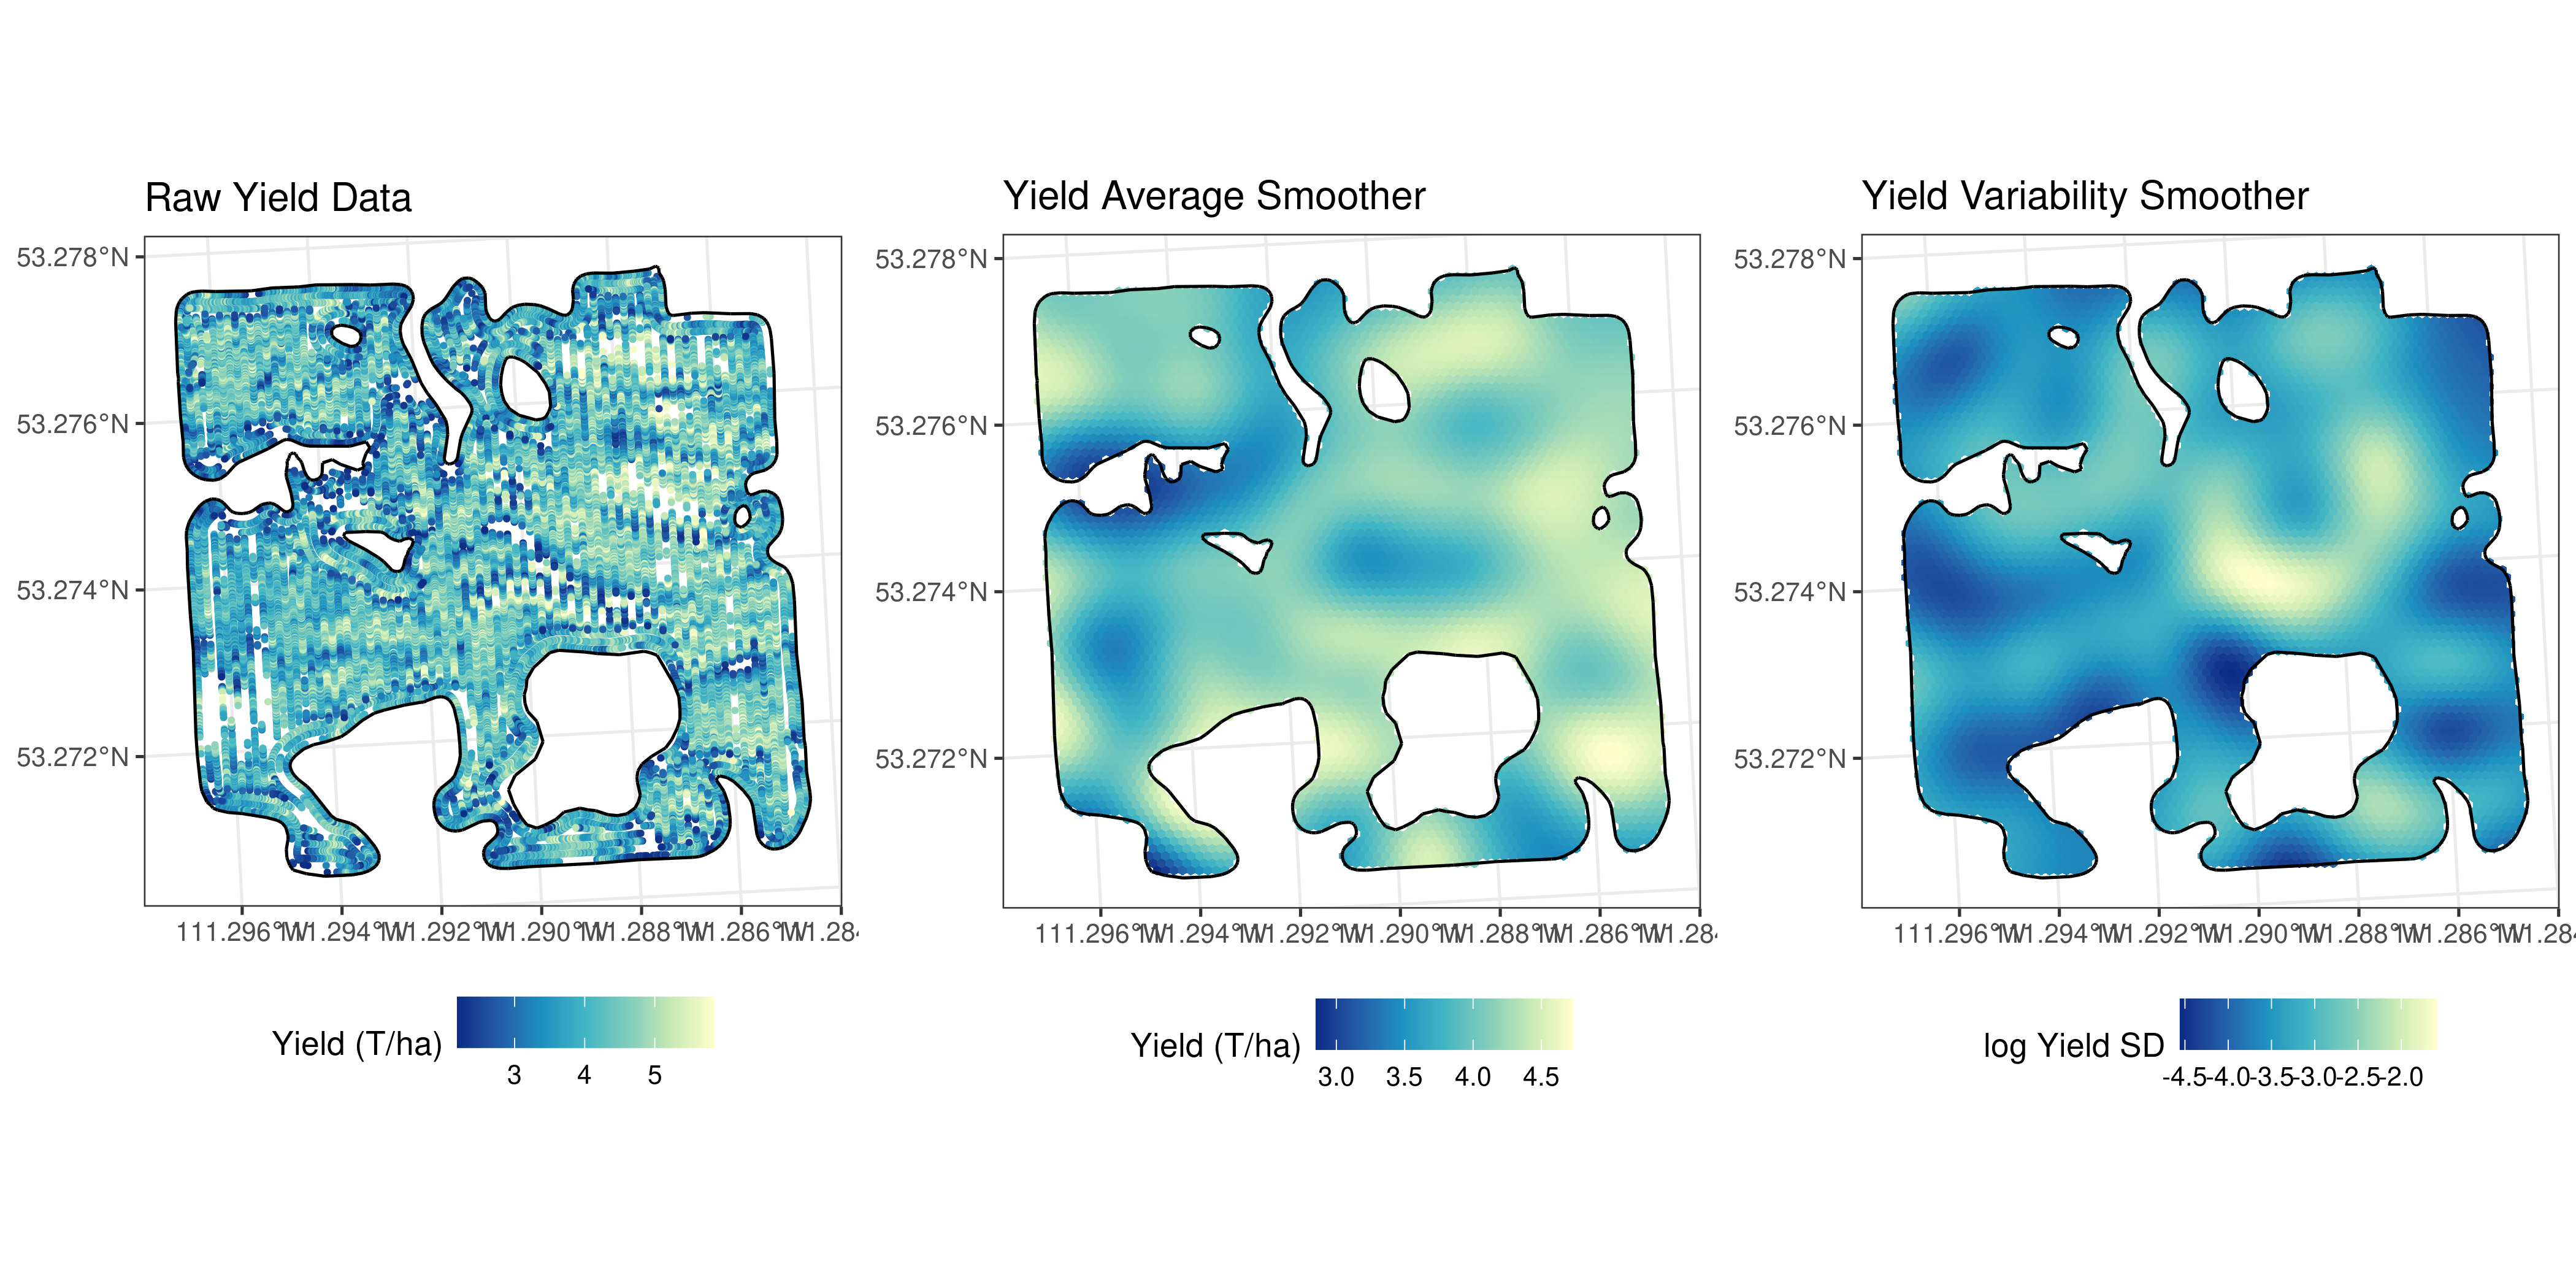
\includegraphics[width=1\linewidth]{../Figures/ExamplePlots/spatialSmooths} \caption{Raw data and spatial smoothers from a single field. Yield averages (means) and variability (log SD) were modeled separately, and both show large spatial dependence within the field.}\label{fig:spatialSmooths}
\end{figure}

\begin{figure}
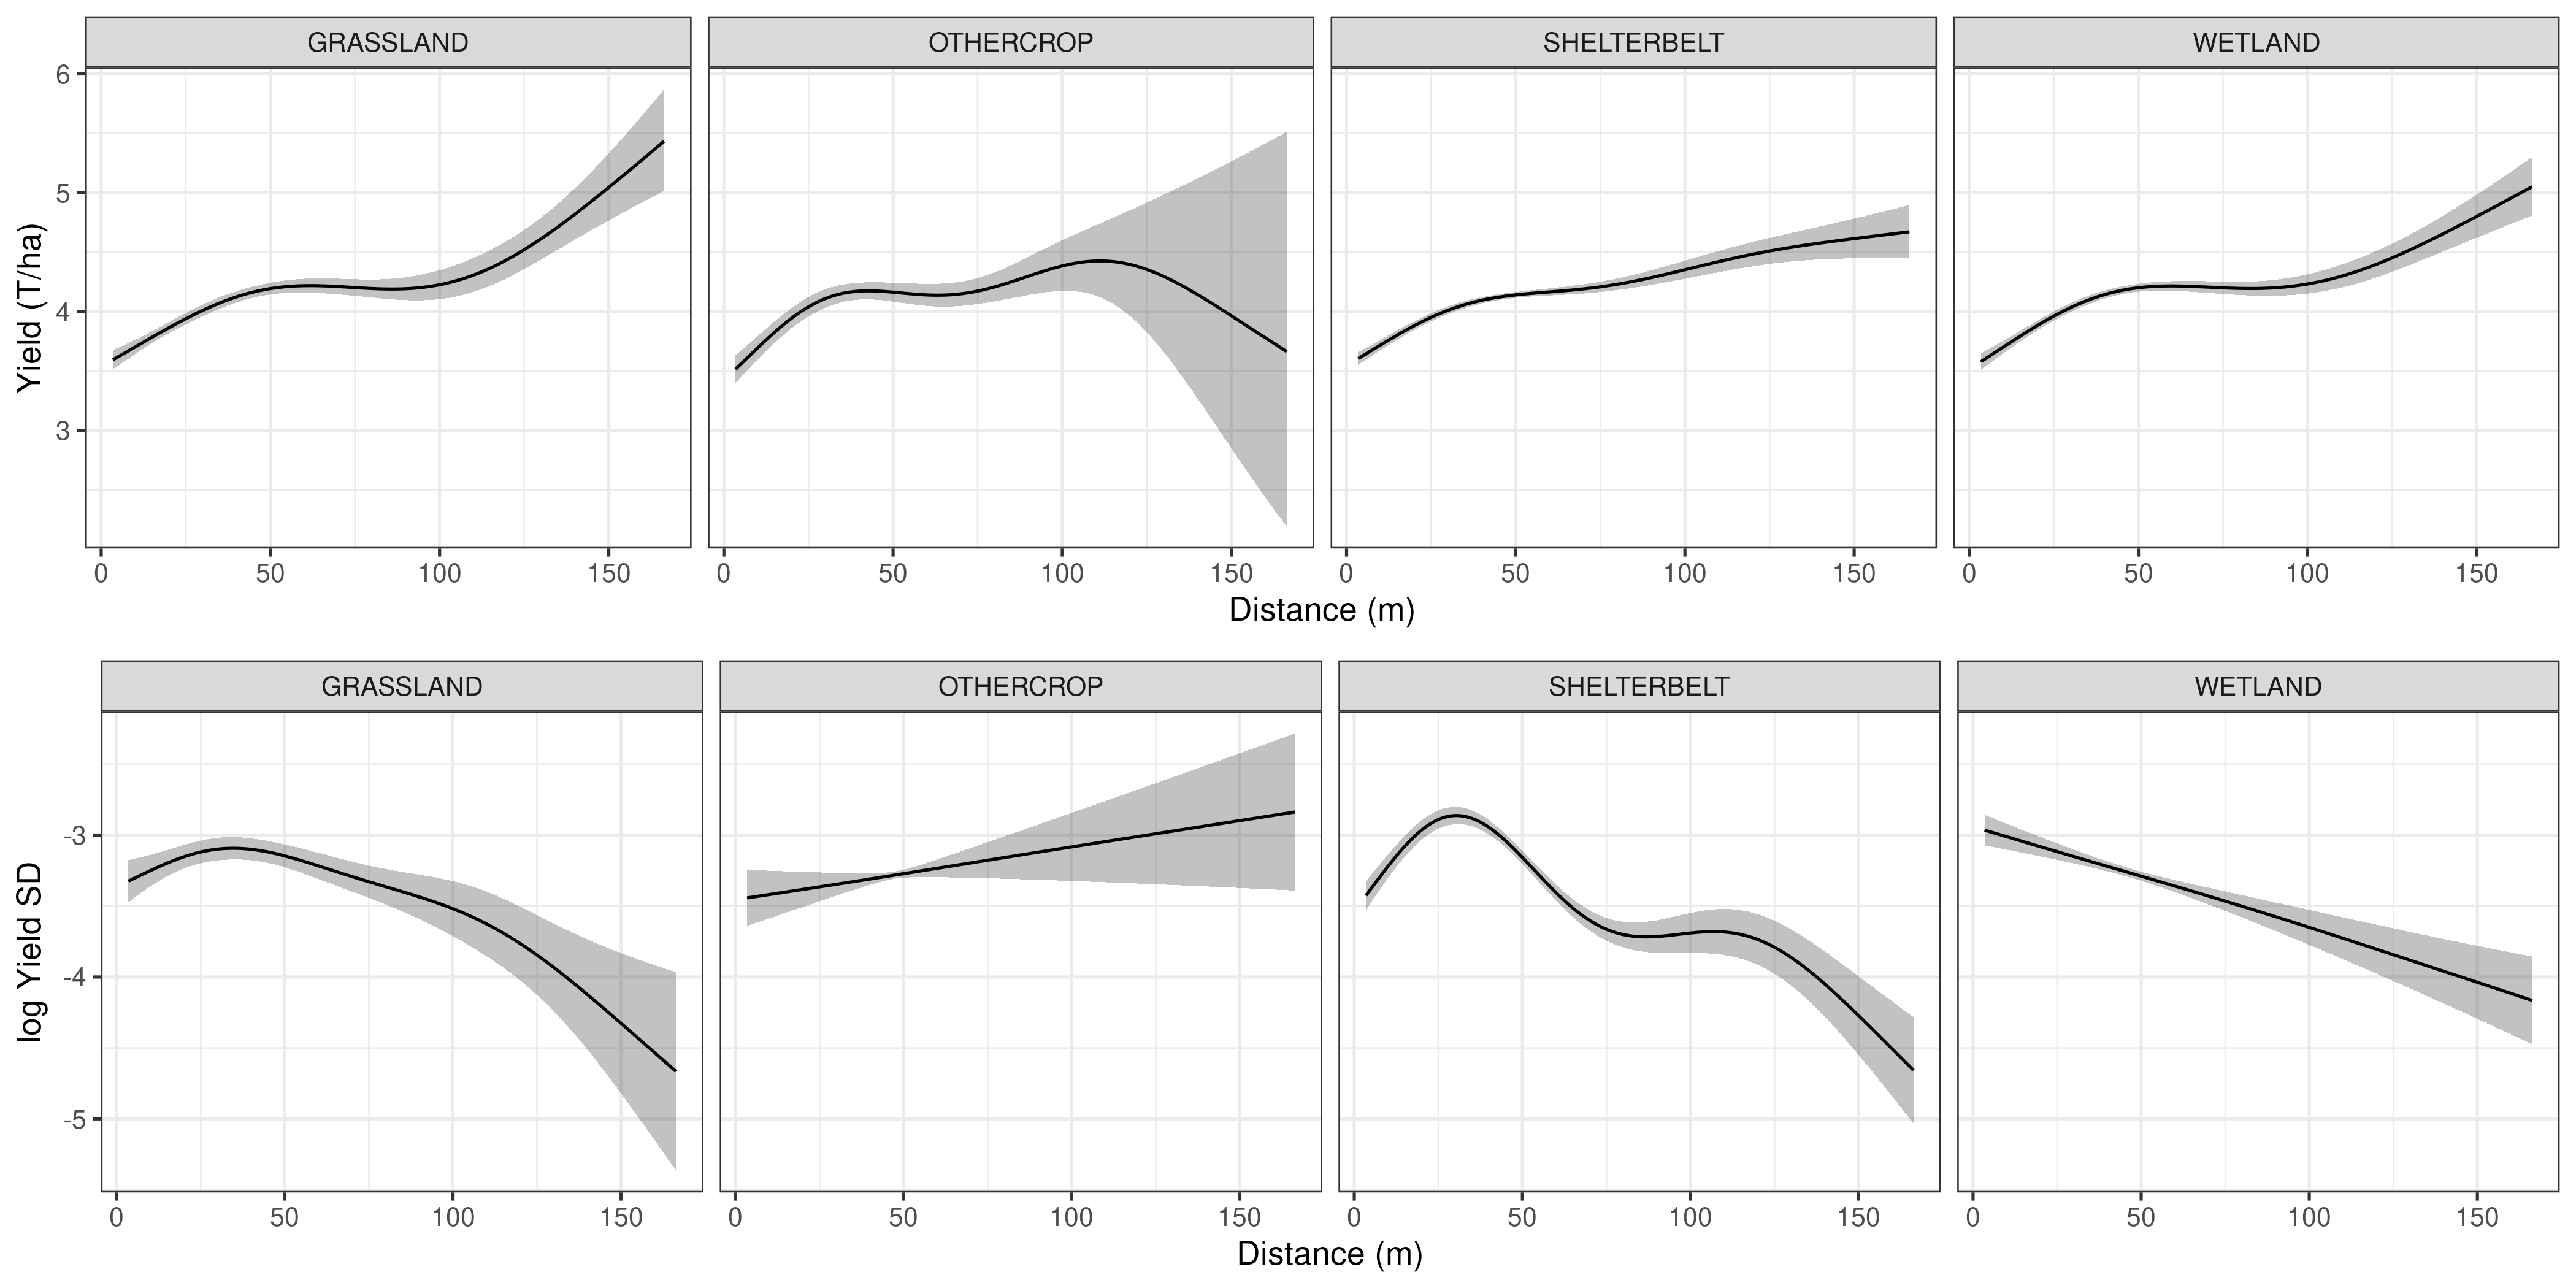
\includegraphics[width=1\linewidth]{../Figures/ExamplePlots/distSmooths} \caption{Distance smoothers from a single field, showing a negative effect of distance on average yield (first row). The variability smoothers show an intermediate reduction in variability at around 90 m.}\label{fig:distSmooths}
\end{figure}

\hypertarget{overall-results}{%
\subsection{Overall results}\label{overall-results}}

Across all fields, standard (grassy border) field boundaries were the most common boundary type, followed by shelterbelts and other crops (Figure \ref{fig:boundaryTypes}).

\begin{figure}
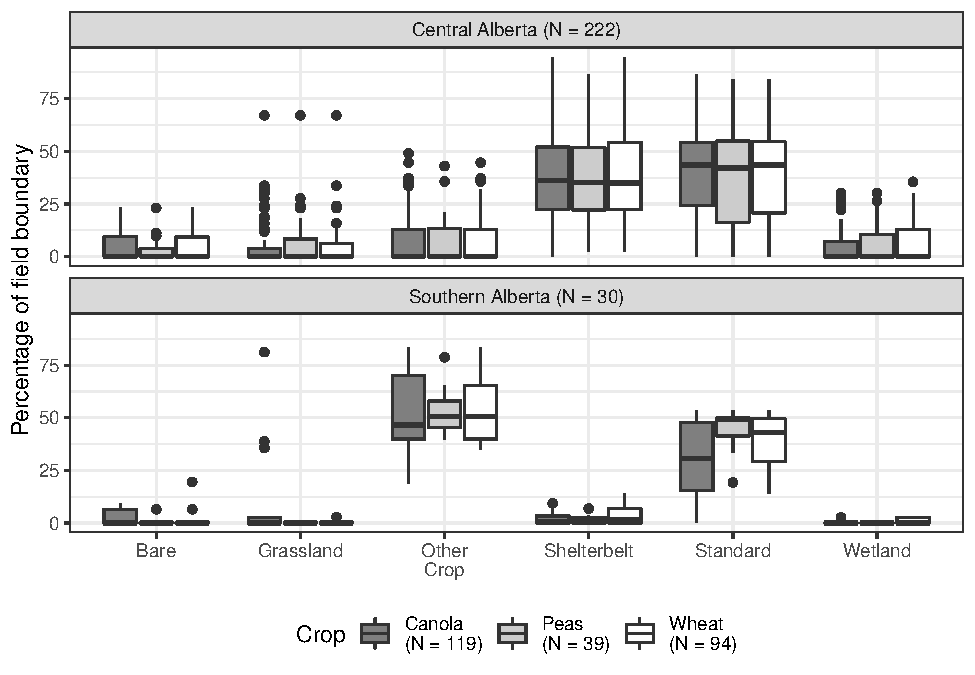
\includegraphics[width=1\linewidth]{manuscript_files/figure-latex/boundaryTypes-1} \caption{Percentage of field boundaries across sampled fields.}\label{fig:boundaryTypes}
\end{figure}

Overall, both yield average and yield variability were extremely spatially dependent across all fields (average p-values both \textless0.0001), meaning that within-field variability was the primary driver of yield across canola, wheat, and pea crops (Table \ref{tab:smoothSummary}, row 6).
Distances from boundary types were also important, but a lower proportion of the fields had strong effects (rows 1-5, cols 3 + 5).

\begin{table}

\caption{\label{tab:smoothSummary}Mean p-values and proportion of p-values less than 0.05 (after Bonneferoni correction) for mean and variability smoothers across all fields.}
\centering
\begin{tabular}[t]{l|r|r|r|r}
\hline
\multicolumn{1}{c|}{} & \multicolumn{2}{c|}{Mean} & \multicolumn{2}{c}{Variability} \\
\cline{2-3} \cline{4-5}
Smoother Type & Average p-value & Proportion <0.05 & Average p-value & Proportion <0.05\\
\hline
Bare & 0.036 & 0.875 & 0.055 & 0.857\\
\hline
Grassland & 0.079 & 0.794 & 0.061 & 0.794\\
\hline
Other Crop & 0.063 & 0.860 & 0.044 & 0.840\\
\hline
Shelterbelt & 0.014 & 0.935 & 0.059 & 0.815\\
\hline
Standard & 0.021 & 0.938 & 0.055 & 0.839\\
\hline
Wetland & 0.045 & 0.833 & 0.013 & 0.857\\
\hline
Spatial Smoother & 0.000 & 1.000 & 0.000 & 1.000\\
\hline
\end{tabular}
\end{table}

Average canola yield tended to increase with distance from all crop boundaries, starting at 2.5 T/ha at the field edge and leveling off at about 3 T/ha (Figure \ref{fig:canolaPlot} top row).
Shelterbelt and standard boundaries were well-represented in the data, and average yield quickly increased with distance away from the field boundary, but shelterbelts had a small intermediate maximum at around 50m before a weak decrease with distance, while average yield away from Standard field boundaries plateaued at 50m and remained roughly constant with distance.
The effect of other boundary types was less consistent, but average yield tended to increase with distance away from grassland, other crop, and wetland, and was roughly the same with distance from bare boundary types.
Yield variability (Figure \ref{fig:canolaPlot} bottom row) was essentially constant with distance for shelterbelt, standard, and other crop field boundaries, but showed some evidence of decreasing with distance from field boundary at wetlands, bare, and grassland.
Interestingly, there was an intermediate reduction in canola yield variability at about 75 m away from Wetland boundaries, indicating a potential stabilizing effect.

\begin{figure}
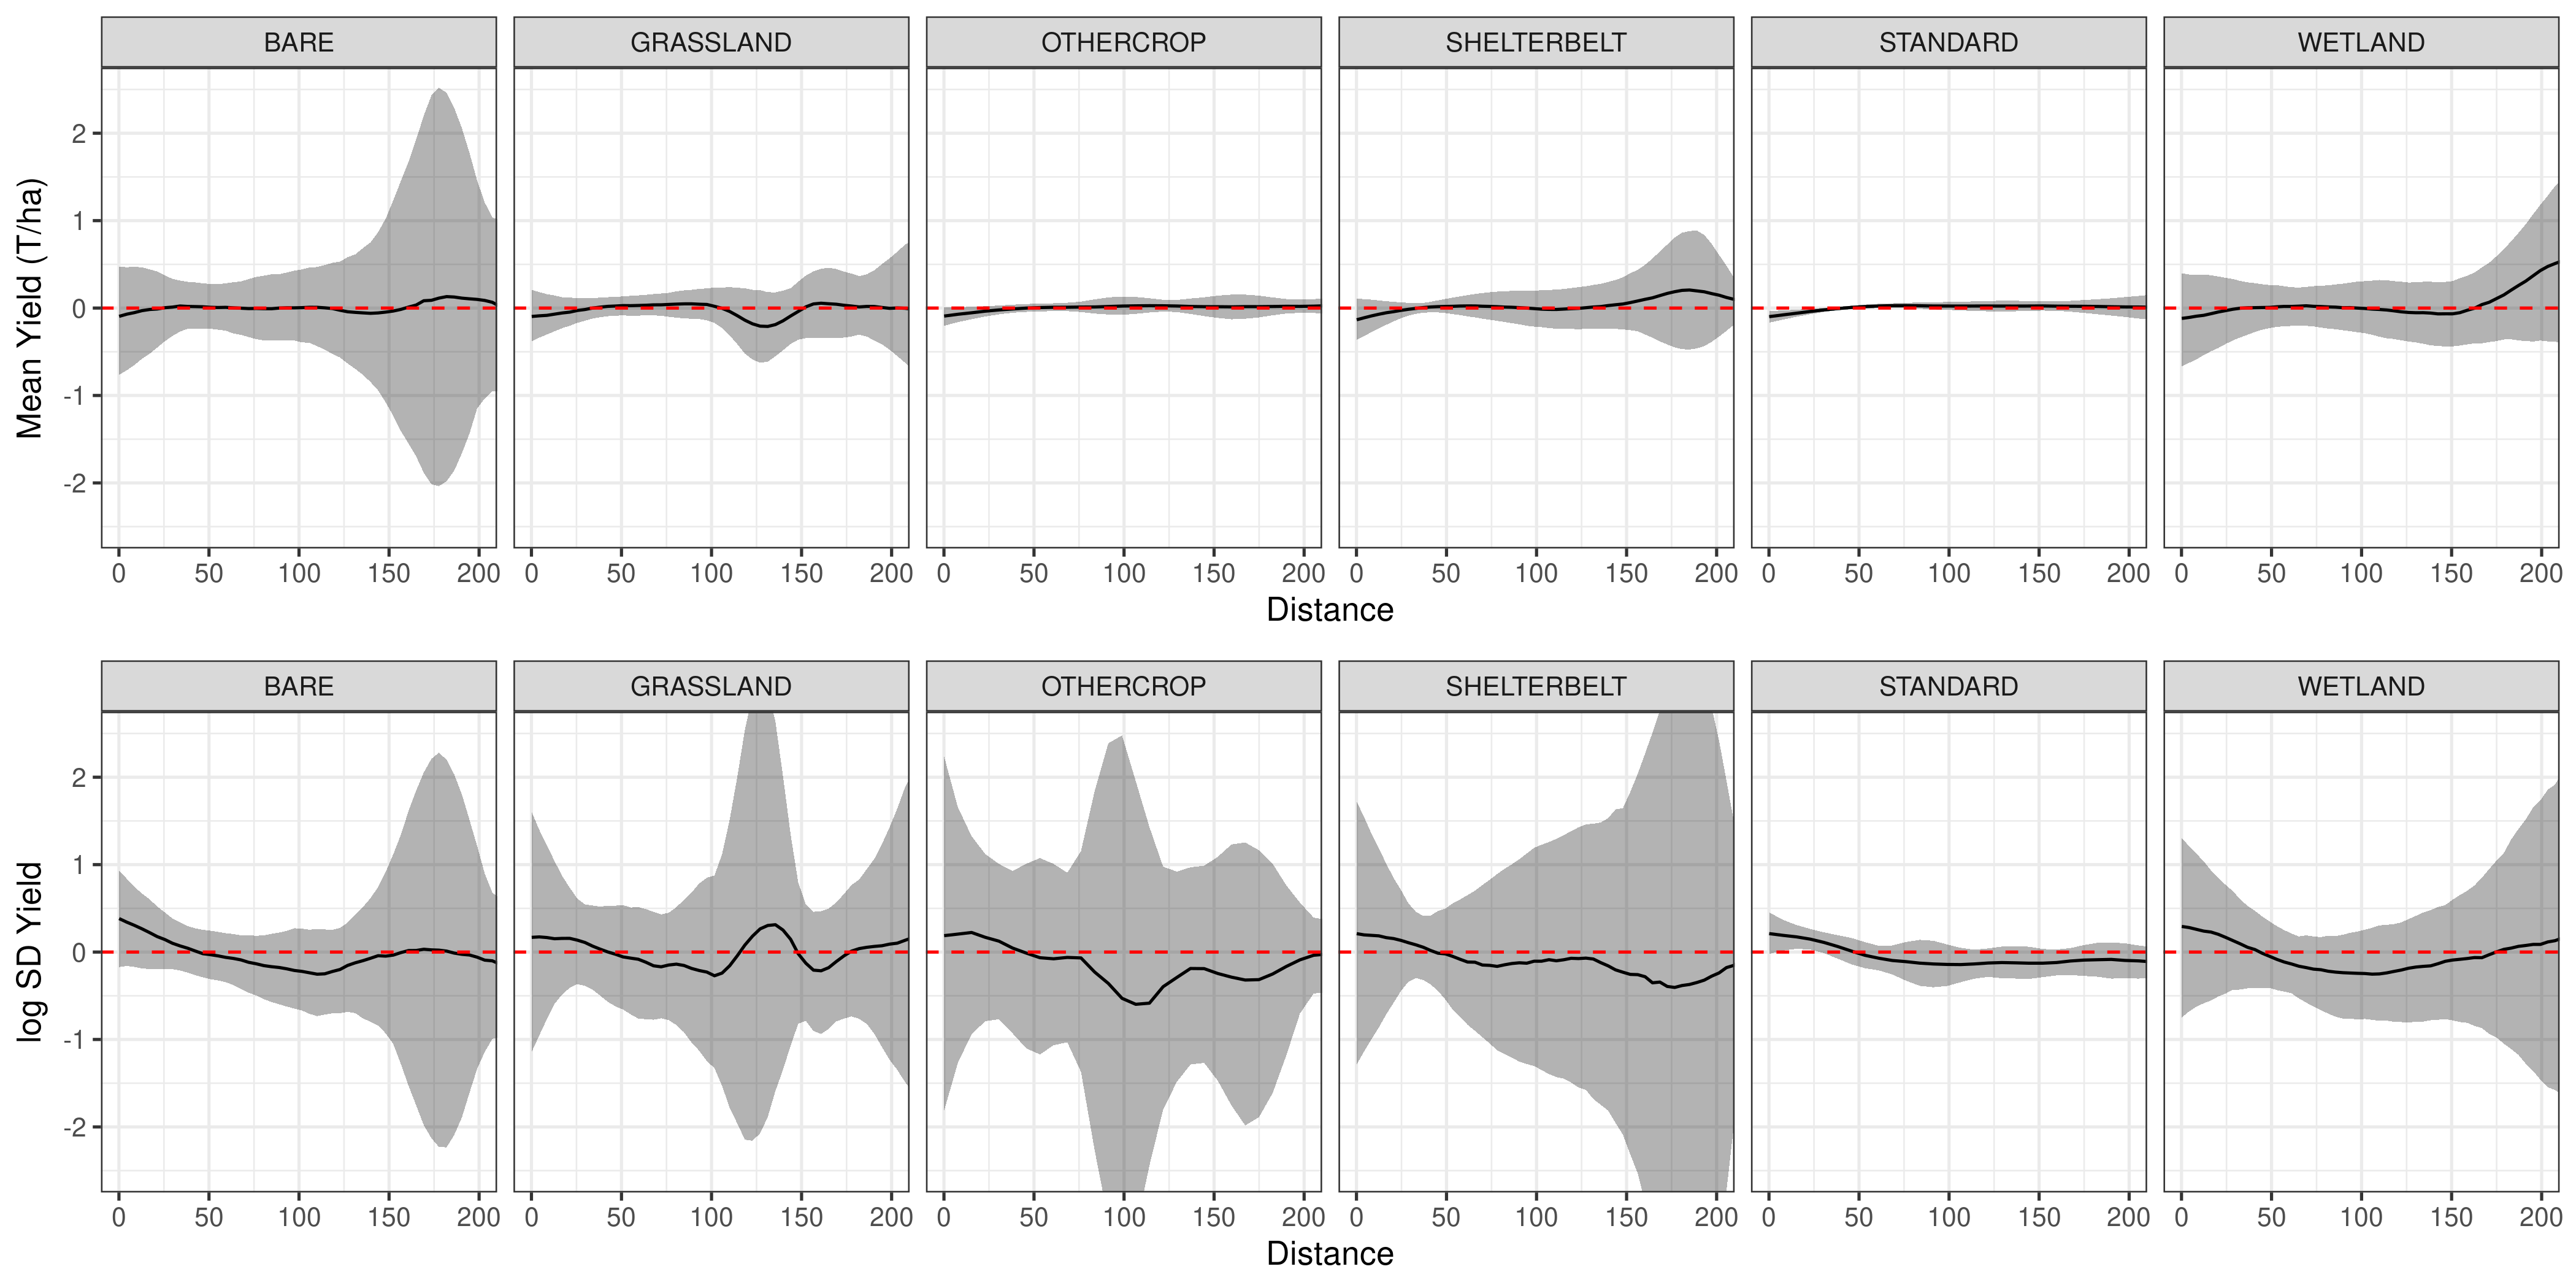
\includegraphics[width=1\linewidth]{../Figures/ModelSummary3a_canola} \caption{Field boundary effect on canola yield, accounting for the effect of spatial variation. Upper panel represents mean yield, while the lower panel represents yield variation. N refers to number of fields containing this boundary type, and \% refers to the average percentage of field boundary accounted for by this boundary type.}\label{fig:canolaPlot}
\end{figure}

The effect of boundary distance on average wheat yield was much more variable than the patterns seen in canola yield.
Average yield (Figure \ref{fig:wheatPlot}, top row) roughly increased with distance away from wetland, standard, and grasslands, but both shelterbelts and bare ground displayed an intermediate maximum at around 50m (similar to canola), and decreased slightly with distance from Other Crops.
Yield variability, on the other hand, tended to decrease with distance from bare, grassland, and wetland (before 100 m, at least), increased slightly with distance from shelterbelt and standard boundaries, and was roughly constant with distance from other crops (Figure \ref{fig:wheatPlot}, bottom row).

\begin{figure}
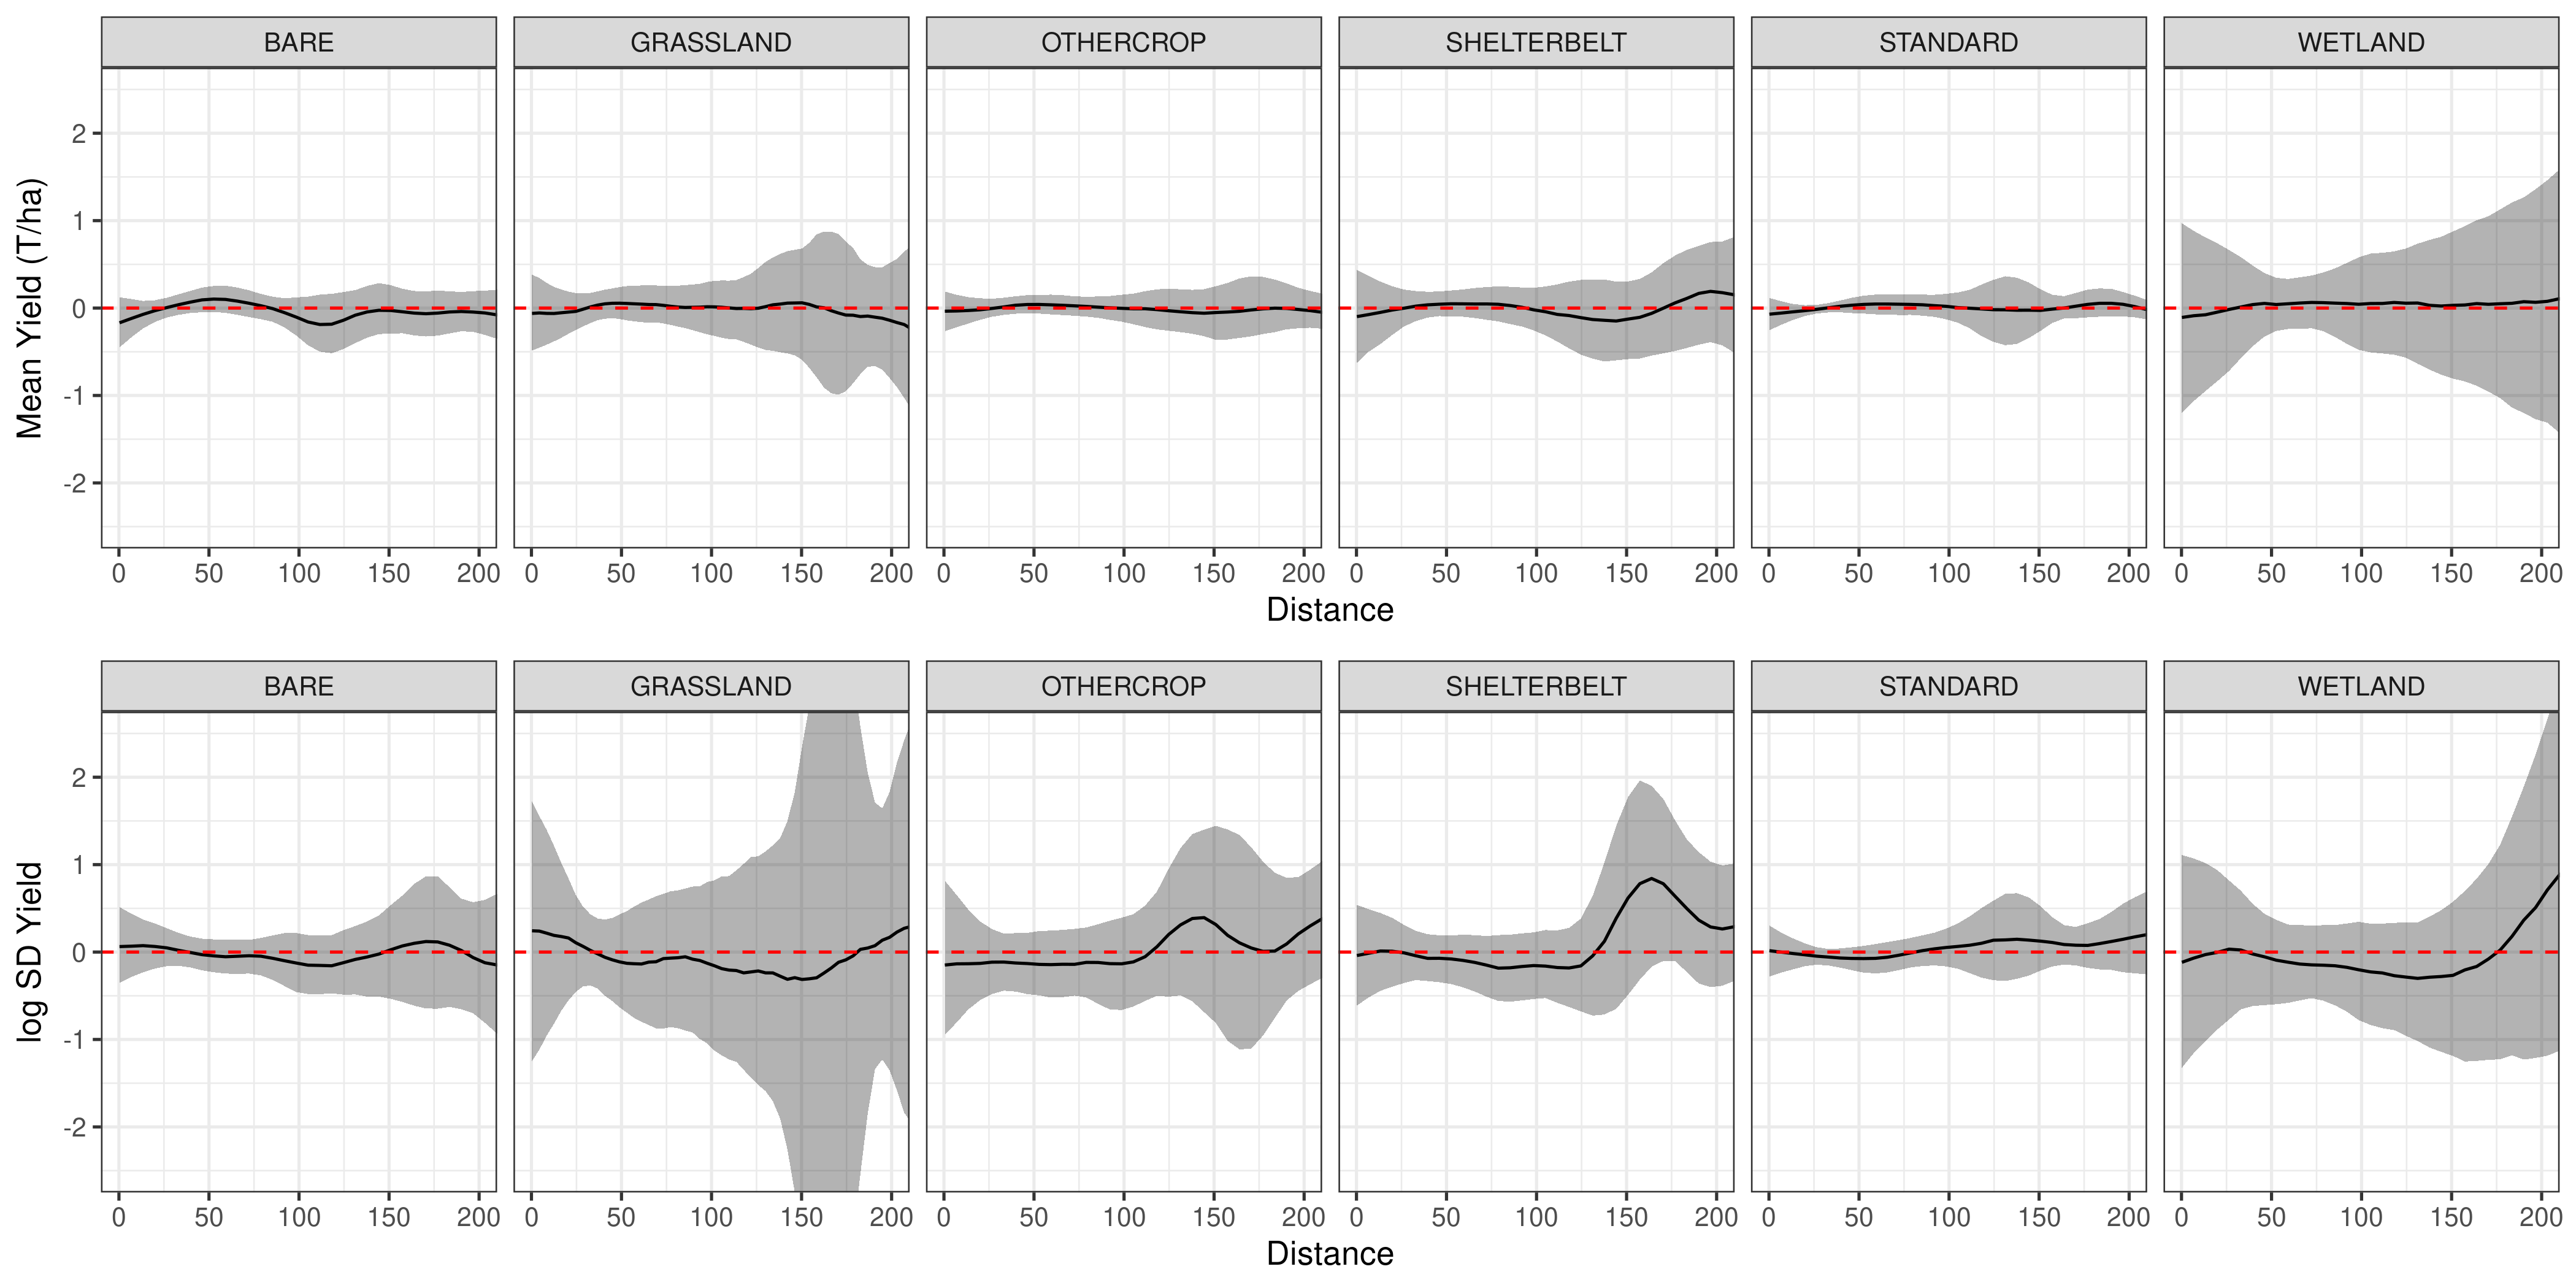
\includegraphics[width=1\linewidth]{../Figures/ModelSummary3a_wheat} \caption{Field boundary effect on wheat yield, accounting for the effect of spatial variation. Upper panel represents mean yield, while the lower panel represents yield variation. N refers to number of fields containing this boundary type, and \% refers to the average percentage of field boundary accounted for by this boundary type.}\label{fig:wheatPlot}
\end{figure}

Pea crops were less well-represented in our data (N = 38 fields, compared to ), and the effects of boundaries tended to be less consistent.
Average pea yields (Figure \ref{fig:peaPlot}, top row) were roughly 4.25 T/ha at the field boundary and increased to just below 5 T/ha away from shelterbelt, standard, and other crop boundaries, while the effect of bare, grassland, and wetland boundaries was inconsistent.
Conversely, yield variability (Figure \ref{fig:peaPlot}, bottom row) decreased with distance from grassland, shelterbelt, standard, and wetland boundaries, while the pattern with distance from other crop and bare was inconsistent.
Unlike canola and wheat crops, there was no obvious evidence of an intermediate increase in yield with distance from the field boundary.

\begin{figure}
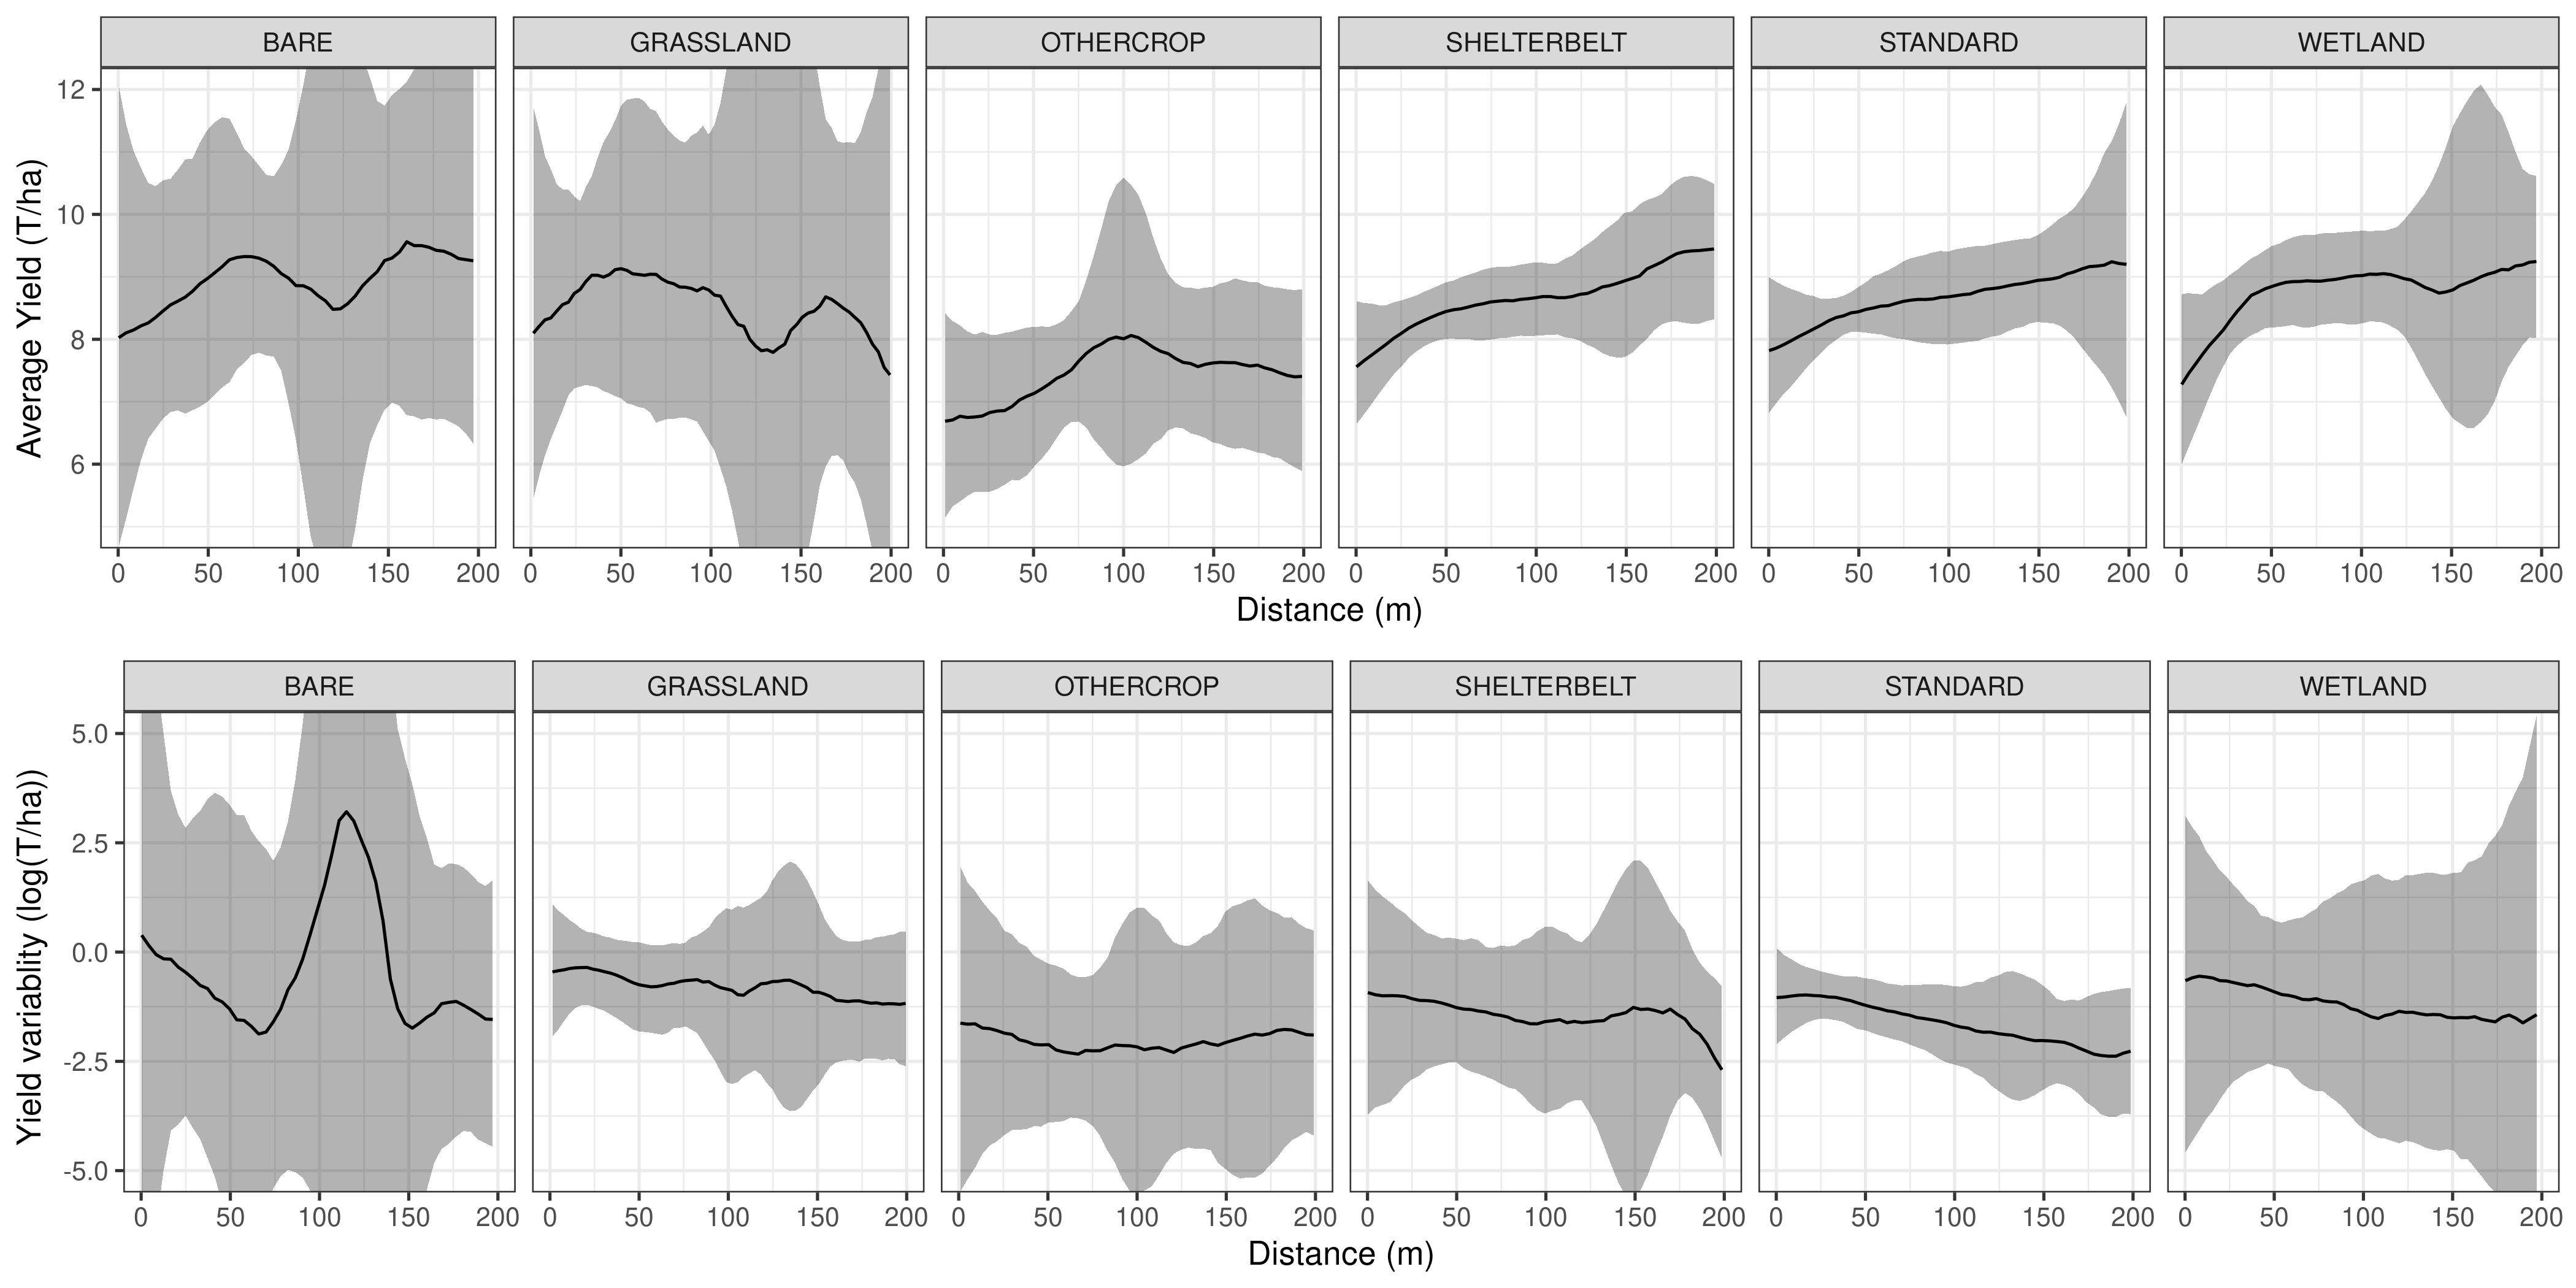
\includegraphics[width=1\linewidth]{../Figures/ModelSummary3a_peas} \caption{Field boundary effect on pea yield, accounting for the effect of spatial variation. Upper panel represents mean yield, while the lower panel represents yield variation. N refers to number of fields containing this boundary type, and \% refers to the average percentage of field boundary accounted for by this boundary type.}\label{fig:peaPlot}
\end{figure}

\hypertarget{discussion}{%
\section{Discussion}\label{discussion}}

At the level of individual fields, both average and variability of yield changed with distance from the field boundary, and there were strong spatial relationships within each field, likely related to underlying soil or moisture conditions.
Yield tended to increase with distance from field boundaries before plateauing, and there was some evidence of intermediate boosts in yield from shelterbelts next to canola and wheat.
This increase tended to be small in magnitude in canola crops, meaning that ecosystem services likely increased or did not vary with distance from field boundaries (Scenario 2, Figure \ref{fig:hypotheses}).
There was a fairly large (0.75 T/ha) intermediate increase in average wheat yields away from shelterbelts, indicating a potential reduction in ecosystem services with distance.
However, there was a similar (albeit weaker) pattern associated with bare ground, so this pattern may be caused by something other than the presence of shelterbelts.
This indicates that shelterbelts may have a positive effect on wheat yields, and future work should expand this across a larger geographic domain in order to inform growers about how best to manage the landscapes surrounding their fields.

Why did we find few consistent effects of boundary type on crop yield, aside from shelterbelts?
Our work examined only the first and last links in the causal chain \emph{Field boundary} \(\rightarrow\) \emph{Insect Abundance} \(\rightarrow\) \emph{Crop Yield}, meaning that are two mediating relationships where the overall relationship could be broken or obscured.
First, field boundaries may not have any influence on insect abundance if separated from the larger landscape context, or spillover of beneficial organisms may be low.
Second, beneficial insect abundance may not influence crop yield if pest pressure or pollination deficits are low, which may vary yearly, or by location.
Our work suggests that we need to better examine the context in which a) beneficial organisms spillover from field boundaries and b) when organisms in crops provide tangible ecosystem services.
We consider these reasons below:

SNL generally has a positive effect on spillover, but field boundaries only represent a fraction of the SNL that surrounds a given field.
Our analysis only examined boundary types, without considering the landscape context that fields were embedded in, but some studies show the influence of landscape composition at larger spatial scales (Nguyen \emph{et al.} 2021) which could be particularly important when beneficial arthropods are disperse very broadly (Öberg \emph{et al.} 2007).
There could also be interactions between landscape composition at different scales (Motzke \emph{et al.} 2016; Haslem \emph{et al.} 2021; Robinson \emph{et al.} 2021), but this is not broadly studied.
Landscape complexity (Fahrig \emph{et al.} 2011) and connectivity are also associated with higher abundance of beneficial arthropods.
This means that field boundaries such as wetlands or shelterbelts may only be helpful if connected to a larger network of non-crop habitat (but see Fahrig \emph{et al.} 2019).

Field boundary traits may play an important role in mediating spillover, but our definitions of boundaries were (necessarily) loose, as we used satellite imagery to manually classify them.
Therefore, it may be that other aspects of field boundaries, such as size or plant community composition, are more important for spillover of ecosystems services into fields.
For example, larger (Lecq \emph{et al.} 2018; Stašiov \emph{et al.} 2020) or more functionally diverse (Bonifacio \emph{et al.} 2011; Boughey \emph{et al.} 2011) hedgerows tend to support more biodiversity than smaller hedgerows, and some studies have shown that leaf litter and soil compaction matters to predatory beetle communities (Sutter \emph{et al.} 2018).
These fine-scale boundary characteristics were not measured in our study, but could be used as variables in more biologically-meaningful classifications of field boundaries.

Our first scenario (Scenario 1, Figure \ref{fig:hypotheses}) assumes that beneficial organisms disperse from boundaries into the field, and had a generally positive effect on crop yield.
However, field boundaries may not have a positive effect if a) ecosystem dis-services -- pest insects or weed seeds -- also disperse along with beneficials, or if b) beneficials do not disperse from the boundary environment.
Pests and weeds can also disperse from field boundaries, which may negate any positive effect of ecosystem services (Zhang \emph{et al.} 2007).
Gray \& Lewis (2014) showed that remnant forest fragments do not provide significant pest control services, but also do not depress yield.
However, this is still poorly studied, and parsing out services from disservices is impossible using crop yield data \emph{alone}.
Ecosystem services from field boundaries may be limited if beneficial organisms stay in field boundaries, or disperse at wider spatial scales Robinson \emph{et al.} (2021).

Pest pressure or pollination deficit may be low enough that ecosystem service provision does not significantly change yield.
Canola is largely self-pollinating (at least in hybrid canola varieties, Lindström \emph{et al.} 2016) and wheat is wind-pollinated, meaning that slight increases in pollination services may not change yields significantly in either crop (Woodcock \emph{et al.} 2016).
Pests are also limited by growers' application of insecticides (seed-treated or on the crop directly), and insect pest outbreaks tend to be temporally and spatially spotty.

Our work is some of the first to use a large precision yield dataset to answer questions about how landscapes influence yield, but this study has only scratched the surface of some of the richest agroecological datasets ever created.
Since our sampling represents a limited amount of spatial and temporal coverage, there could be additional confounding variables that obscure signals of yield.
Most fields were located in Central Alberta (Dry Mixedwood region, Natural Regions Committee 2006), where boundaries contained a higher proportion of shelterbelts (Figure \ref{fig:boundaryTypes}), but differences from Southern AB (Foothills Fescue and Mixedgrass region) may be confounding the signal.
Between-year effects may be important, especially during dry years (Kort 1988), but this was not considered in our analysis.
Future work could examine whether boundaries have differing effects during hot or cool years, as shading or cooling effects may increase yield during hot years but have negative (or no) effect during cooler years.

\hypertarget{author-contributions}{%
\section{Author Contributions}\label{author-contributions}}

SVJR, LHN, and PG conceived of the project.
SVJR collected data, conducted analysis, and wrote the manuscript.

\hypertarget{acknowledgements}{%
\section{Acknowledgements}\label{acknowledgements}}

We thank Trent Clark, Dean Hubbard, Alvin French, and Kristina Polziehn for providing yield data for us, and providing insight on their yield data.
We also thank Autumn Barnes and Keith Gabert of the Canola Council of Canada, and Laurel Thompson and JP Pettyjohn of Lakeland College for connecting us with farmers and agronomists.
Funding for this research was provided by Ducks Unlimited Canada's Institute for Wetland and Waterfowl Research, the Alberta Canola Producers Commission, Manitoba Canola Growers Association, SaskCanola, the Alberta Biodiversity Monitoring Institute, and the Alberta Conservation Association.

\hypertarget{references}{%
\section*{References}\label{references}}
\addcontentsline{toc}{section}{References}

\hypertarget{refs}{}
\begin{CSLReferences}{1}{0}
\leavevmode\hypertarget{ref-albrecht2020}{}%
Albrecht, M., Kleijn, D., Williams, N.M., Tschumi, M., Blaauw, B.R., Bommarco, R., \emph{et al.} (2020). The effectiveness of flower strips and hedgerows on pest control, pollination services and crop yield: A quantitative synthesis. \emph{Ecology Letters}.

\leavevmode\hypertarget{ref-arslan2002}{}%
Arslan, S. \& Colvin, T.S. (2002). An evaluation of the response of yield monitors and combines to varying yields. \emph{Precision Agriculture}, 3, 107--122.

\leavevmode\hypertarget{ref-baker2018}{}%
Baker, T.P., Moroni, M.T., Mendham, D.S., Smith, R. \& Hunt, M.A. (2018). Impacts of windbreak shelter on crop and livestock production. \emph{Crop and Pasture Science}, 69, 785.

\leavevmode\hypertarget{ref-boetzl2020}{}%
Boetzl, F.A., Schuele, M., Krauss, J. \& Steffan-Dewenter, I. (2020). Pest control potential of adjacent agri-environment schemes varies with crop type and is shaped by landscape context and within-field position. \emph{Journal of Applied Ecology}, 57, 1482--1493.

\leavevmode\hypertarget{ref-bonifacio2011}{}%
Bonifacio, R.S., Kinross, C.M., Gurr, G.M. \& Nicol, H. (2011). The effect of woody plant diversity and other stand and landscape factors on the diversity and abundance of birds using farm shelterbelts. \emph{Pacific Conservation Biology}, 17, 22.

\leavevmode\hypertarget{ref-boughey2011}{}%
Boughey, K.L., Lake, I.R., Haysom, K.A. \& Dolman, P.M. (2011). Improving the biodiversity benefits of hedgerows: How physical characteristics and the proximity of foraging habitat affect the use of linear features by bats. \emph{Biological Conservation}, 144, 1790--1798.

\leavevmode\hypertarget{ref-brandle2004}{}%
Brandle, J.R., Hodges, L. \& Zhou, X.H. (2004). Windbreaks in {North American} agricultural systems. In: \emph{New vistas in agroforestry: A compendium for 1st world congress of agroforestry, 2004} (eds. Nair, P.K.R., Rao, M.R. \& Buck, L.E.). Springer Netherlands, Dordrecht, pp. 65--78.

\leavevmode\hypertarget{ref-case2019}{}%
Case, B.S., Pannell, J.L., Stanley, M.C., Norton, D.A., Brugman, A., Funaki, M., \emph{et al.} (2019). Non-production vegetation has a positive effect on ecological processes in agroecosystems. \emph{bioRxiv}, 624635.

\leavevmode\hypertarget{ref-cressie2011}{}%
Cressie, N. \& Wikle, C.K. (2011). \emph{Statistics for spatio-temporal data}. Wiley.

\leavevmode\hypertarget{ref-duelli2003}{}%
Duelli, P. \& Obrist, M.K. (2003). Regional biodiversity in an agricultural landscape: The contribution of seminatural habitat islands. \emph{Basic and Applied Ecology}, 4, 129--138.

\leavevmode\hypertarget{ref-fahrig2019}{}%
Fahrig, L., Arroyo-Rodríguez, V., Bennett, J.R., Boucher-Lalonde, V., Cazetta, E., Currie, D.J., \emph{et al.} (2019). Is habitat fragmentation bad for biodiversity? \emph{Biological Conservation}, 230, 179--186.

\leavevmode\hypertarget{ref-fahrig2011}{}%
Fahrig, L., Baudry, J., Brotons, L., Burel, F.G., Crist, T.O., Fuller, R.J., \emph{et al.} (2011). Functional landscape heterogeneity and animal biodiversity in agricultural landscapes. \emph{Ecology Letters}, 14, 101--112.

\leavevmode\hypertarget{ref-foley2011}{}%
Foley, J.A., Ramankutty, N., Brauman, K.A., Cassidy, E.S., Gerber, J.S., Johnston, M., \emph{et al.} (2011). Solutions for a cultivated planet. \emph{Nature}, 478, 337--342.

\leavevmode\hypertarget{ref-frei2018}{}%
Frei, B., Renard, D., Mitchell, M.G.E., Seufert, V., Chaplin-Kramer, R., Rhemtulla, J.M., \emph{et al.} (2018). Bright spots in agricultural landscapes: Identifying areas exceeding expectations for multifunctionality and biodiversity. \emph{Journal of Applied Ecology}, 55, 2731--2743.

\leavevmode\hypertarget{ref-gardner2021}{}%
Gardner, E., Breeze, T.D., Clough, Y., Smith, H.G., Baldock, K.C.R., Campbell, A., \emph{et al.} (2021). Field boundary features can stabilise bee populations and the pollination of mass-flowering crops in rotational systems. \emph{Journal of Applied Ecology}, In press.

\leavevmode\hypertarget{ref-garibaldi2011}{}%
Garibaldi, L.A., Steffan-Dewenter, I., Kremen, C., Morales, J.M., Bommarco, R., Cunningham, S.A., \emph{et al.} (2011). Stability of pollination services decreases with isolation from natural areas despite honey bee visits. \emph{Ecology Letters}, 14, 1062--1072.

\leavevmode\hypertarget{ref-gray2014}{}%
Gray, C.L. \& Lewis, O.T. (2014). Do riparian forest fragments provide ecosystem services or disservices in surrounding oil palm plantations? \emph{Basic and Applied Ecology}, 15, 693--700.

\leavevmode\hypertarget{ref-griffin2007}{}%
Griffin, T.W., Brown, J.P. \& Lowenberg-DeBoerc, J. (2007). \emph{Yield monitor data analysis protocol: A primer in the management and analysis of precision agriculture data}.

\leavevmode\hypertarget{ref-haslem2021}{}%
Haslem, A., Clarke, R.H., Holland, G.J., Radford, J.Q., Stewart, A. \& Bennett, A.F. (2021). Local management or wider context: What determines the value of farm revegetation plantings for birds? \emph{Journal of Applied Ecology}.

\leavevmode\hypertarget{ref-hunicken2021}{}%
Hünicken, P.L., Morales, C.L., Aizen, M.A., Anderson, G.K.S., García, N. \& Garibaldi, L.A. (2021). Insect pollination enhances yield stability in two pollinator-dependent crops. \emph{Agriculture, Ecosystems {\&} Environment}, 320, 107573.

\leavevmode\hypertarget{ref-kassambara2020}{}%
Kassambara, A. (2020). \emph{{ggpubr}: 'ggplot2' based publication ready plots}.

\leavevmode\hypertarget{ref-kort1988}{}%
Kort, J. (1988). 9. Benefits of windbreaks to field and forage crops. \emph{Agriculture, Ecosystems {\&} Environment}, 22-23, 165--190.

\leavevmode\hypertarget{ref-kowalchuk1995}{}%
Kowalchuk, T.E. \& Jong, E. de. (1995). Shelterbelts and their effect on crop yield. \emph{Canadian Journal of Soil Science}, 75, 543--550.

\leavevmode\hypertarget{ref-lecq2018}{}%
Lecq, S., Loisel, A., Mullin, S.J. \& Bonnet, X. (2018). Manipulating hedgerow quality: Embankment size influences animal biodiversity in a peri-urban context. \emph{Urban Forestry {\&} Urban Greening}, 35, 1--7.

\leavevmode\hypertarget{ref-lindstrom2016}{}%
Lindström, S.A.M., Herbertsson, L., Rundlöf, M., Smith, H.G. \& Bommarco, R. (2016). Large-scale pollination experiment demonstrates the importance of insect pollination in winter oilseed rape. \emph{Oecologia}, 180, 759--769.

\leavevmode\hypertarget{ref-lowe2021}{}%
Lowe, E.B., Groves, R. \& Gratton, C. (2021). Impacts of field-edge flower plantings on pollinator conservation and ecosystem service delivery {{}} a meta-analysis. \emph{Agriculture, Ecosystems {\&} Environment}, 310, 107290.

\leavevmode\hypertarget{ref-marja2019}{}%
Marja, R., Kleijn, D., Tscharntke, T., Klein, A.-M., Frank, T. \& Batáry, P. (2019). Effectiveness of agri-environmental management on pollinators is moderated more by ecological contrast than by landscape structure or land-use intensity. \emph{Ecology Letters}, In press.

\leavevmode\hypertarget{ref-mitchell2014}{}%
Mitchell, M.G.E., Bennett, E.M. \& Gonzalez, A. (2014). Forest fragments modulate the provision of multiple ecosystem services. \emph{Journal of Applied Ecology}, 51, 909--918.

\leavevmode\hypertarget{ref-motzke2016}{}%
Motzke, I., Klein, A.-M., Saleh, S., Wanger, T.C. \& Tscharntke, T. (2016). Habitat management on multiple spatial scales can enhance bee pollination and crop yield in tropical homegardens. \emph{Agriculture, Ecosystems \& Environment}, 223, 144--151.

\leavevmode\hypertarget{ref-ABRegions2006}{}%
Natural Regions Committee. (2006). \emph{Natural regions and subregions of {Alberta}}. Government of Alberta, Edmonton.

\leavevmode\hypertarget{ref-nguyen2021}{}%
Nguyen, L.H., Robinson, S.V.J. \& Galpern, P. (2021). Medium-resolution multispectral satellite imagery in precision agriculture: Mapping precision canola (\emph{brassica napus} {L.}) Yield using {Sentinel-2} time series. \emph{Precision Agriculture}, In Review (Preprint: https://www.essoar.org/doi/10.1002/essoar.10507479.2).

\leavevmode\hypertarget{ref-oberg2007}{}%
Öberg, S., Ekbom, B. \& Bommarco, R. (2007). Influence of habitat type and surrounding landscape on spider diversity in {Swedish} agroecosystems. \emph{Agriculture, Ecosystems {\&} Environment}, 122, 211--219.

\leavevmode\hypertarget{ref-prietoBenitez2011}{}%
Prieto-Benítez, S. \& Méndez, M. (2011). Effects of land management on the abundance and richness of spiders ({Araneae}): A meta-analysis. \emph{Biological Conservation}, 144, 683--691.

\leavevmode\hypertarget{ref-quinn2017}{}%
Quinn, N.F., Brainard, D.C. \& Szendrei, Z. (2017). Floral strips attract beneficial insects but do not enhance yield in cucumber fields. \emph{Journal of Economic Entomology}, 110, 517--524.

\leavevmode\hypertarget{ref-ramankutty2018}{}%
Ramankutty, N., Mehrabi, Z., Waha, K., Jarvis, L., Kremen, C., Herrero, M., \emph{et al.} (2018). Trends in global agricultural land use: Implications for environmental health and food security. \emph{Annual Review of Plant Biology}, 69, 789--815.

\leavevmode\hypertarget{ref-redhead2020}{}%
Redhead, J.W., Oliver, T.H., Woodcock, B.A. \& Pywell, R.F. (2020). The influence of landscape composition and configuration on crop yield resilience. \emph{Journal of Applied Ecology}, 57, 2180--2190.

\leavevmode\hypertarget{ref-robinson2021}{}%
Robinson, S.V.J., Edwards, D., Vickruck, J.L., Best, L.R. \& Galpern, P. (2021). Non-crop sources of beneficial arthropods vary within-season across a prairie agroecosystem. \emph{Agriculture, Ecosystems {\&} Environment}, 320, 107581.

\leavevmode\hypertarget{ref-stasiov2020}{}%
Stašiov, S., Diviaková, A., Svitok, M., Novikmec, M. \& Dovciak, M. (2020). Hedgerows support rich communities of harvestmen ({Opiliones}) in upland agricultural landscape. \emph{Basic and Applied Ecology}, 47, 73--82.

\leavevmode\hypertarget{ref-statscan_canola2014}{}%
Statistics Canada. (2014). Table 001-0010 - estimated areas, yield, production and average farm price of principal field crops, in metric units, annual.

\leavevmode\hypertarget{ref-sutter2018b}{}%
Sutter, L., Amato, M., Jeanneret, P. \& Albrecht, M. (2018). Overwintering of pollen beetles and their predators in oilseed rape and semi-natural habitats. \emph{Agriculture, Ecosystems {\&} Environment}, 265, 275--281.

\leavevmode\hypertarget{ref-vanVooren2017}{}%
Van Vooren, L., Bert, R., Steven, B., Pieter, D.F., Victoria, N., Paul, P., \emph{et al.} (2017). Ecosystem service delivery of agri-environment measures: A synthesis for hedgerows and grass strips on arable land. \emph{Agriculture, Ecosystems {\&} Environment}, 244, 32--51.

\leavevmode\hypertarget{ref-vega2019}{}%
Vega, A., Córdoba, M., Castro-Franco, M. \& Balzarini, M. (2019). Protocol for automating error removal from yield maps. \emph{Precision Agriculture}, 20, 1030--1044.

\leavevmode\hypertarget{ref-weninger2021}{}%
Weninger, T., Scheper, S., Lackóová, L., Kitzler, B., Gartner, K., King, N.W., \emph{et al.} (2021). Ecosystem services of tree windbreaks in rural landscapes -- a systematic review. \emph{Environmental Research Letters}, In press.

\leavevmode\hypertarget{ref-whelan2013}{}%
Whelan, B. \& Taylor, J. (2013). \emph{Precision agriculture for grain production systems}. CSIRO Publishing.

\leavevmode\hypertarget{ref-wickham2016}{}%
Wickham, H. (2016). \emph{{ggplot2}: Elegant graphics for data analysis}. Springer-Verlag New York.

\leavevmode\hypertarget{ref-wickle2019}{}%
Wikle, C.K., Zammit-Mangion, A. \& Cressie, N. (2019). \emph{Spatio-temporal statistics with r}. Chapman; Hall: CRC Press.

\leavevmode\hypertarget{ref-wood2017}{}%
Wood, S.N. (2017). \emph{Generalized additive models: An introduction with {R}}. CRC press.

\leavevmode\hypertarget{ref-woodcock2016}{}%
Woodcock, B.A., Bullock, J.M., McCracken, M., Chapman, R.E., Ball, S.L., Edwards, M.E., \emph{et al.} (2016). Spill-over of pest control and pollination services into arable crops. \emph{Agriculture, Ecosystems \& Environment}, 231, 15--23.

\leavevmode\hypertarget{ref-wratten2012}{}%
Wratten, S.D., Gillespie, M., Decourtye, A., Mader, E. \& Desneux, N. (2012). Pollinator habitat enhancement: Benefits to other ecosystem services. \emph{Agriculture, Ecosystems {\&} Environment}, 159, 112--122.

\leavevmode\hypertarget{ref-zamorano2020}{}%
Zamorano, J., Bartomeus, I., Grez, A.A. \& Garibaldi, L.A. (2020). Field margin floral enhancements increase pollinator diversity at the field edge but show no consistent spillover into the crop field: A meta-analysis. \emph{Insect Conservation and Diversity}, 13, 519--531.

\leavevmode\hypertarget{ref-zhang2007}{}%
Zhang, W., Ricketts, T.H., Kremen, C., Carney, K. \& Swinton, S.M. (2007). Ecosystem services and dis-services to agriculture. \emph{Ecological Economics}, 64, 253--260.

\end{CSLReferences}


\end{document}

